In this section, we present our program analysis {\THESYSTEM} for
computing an upper bound on the \emph{adaptivity} of a given program
$c$.  The high level idea behind {\THESYSTEM} is to first build
an \emph{estimated dependency graph} \progG(c) of a program $c$
(Section~\ref{sec:alg_weightedgegen}) which overapproximates the
semantics-based dependency graph in two dimensions: it
overapproximates the dependencies between assigned variables (Section~\ref{sec:alg_edgegen}), and, it
overapproximates the weights (Section~\ref{sec:alg_weightgen}). Then, {\THESYSTEM} uses a custom algorithm to estimate the longest
walk on this graph, providing in this way an upper bound on the adaptivity of the
program.
%
\subsection{A guide to {\THESYSTEM}}
\label{sec:alg_guide}
In order to have a sound and accurate upper bound on the  adaptivity of a program $c$,
we design a program analysis framework named {\THESYSTEM}.
This framework composes two algorithms as shown in the double-stroke box and the dashed box in Fig.~\ref{fig:adaptfun}.
The first algorithm in the double-stroke box combines the quantitative and dependency analysis techniques.
It produces an estimated \emph{data-dependency graph} for a program.
The second algorithm in the dashed box is a walk length estimation algorithm.
%  in the dashed box in Fig.~\ref{fig:adaptfun}.
It computes the upper bound on the program's \emph{adaptivity} over the estimated graph.
%  of the adaptive data analysis program $c$.
\begin{figure}
  \centering    
\includegraphics[width=1.0\columnwidth]{adaptfun.png}
  \vspace{-0.3cm}
  \caption{The overview of {\THESYSTEM}}
  \label{fig:adaptfun}
  \vspace{-0.5cm}
\end{figure}
%
Below is the outline of the {\THESYSTEM}.
% through Section~\ref{sec:alg_vertexgen}, Section~\ref{sec:alg_weightedgegen} and~\ref{sec:alg_graphgen}:
\begin{enumerate}
  \item \textbf{Graph Estimation}
  Because adaptivity is defined over a program's \emph{quantitative dependency graph} (in Definition~\ref{def:trace_graph}),
  this algorithm first estimates this graph for the program statically
  in Section~\ref{sec:alg_graphgen}.
  It estimates the four components of this graph in two steps and then composes them into an estimated dependency graph
  %  for a program 
  in the last step.
  The steps are summarized  as follows.
\begin{enumerate}
  \item \textbf{Vertex and Query Annotation Estimation}
  Vertices and query annotations in this graph are the assigned variables with unique labels. These are extracted directly from the program as in Section~\ref{sec:alg_vertexgen}.
  \item \textbf{Edge and Weight Estimation}
  \\
  This step estimates the edge and weight for a quantitative dependency graph. It combines the control, data-flow  analysis algorithm and the loop bound inference algorithm.
  There are three computation steps in this algorithm.
  \\
  \textbf{Abstract Control Flow Graph.}
  In order to perform the dependency analysis and quantitative analysis, this step first generates an \emph{abstract control flow graph} for a program in Section~\ref{sec:alg_abscfg}.
  \\
  \textbf{Edges Estimation via Combined Flow Analysis.} 
  The step is presented in
  Section~\ref{sec:alg_edgegen}. It performs over the \emph{abstract control flow graph}, which combines both control flow and data flow analysis.
  It estimates the \emph{dependency relation} between each pair of the labeled variables in a program by considering both the control flow and data flow.
  Then it uses the estimated dependency relation to approximate the edge
  %  of the quantitative dependency graph 
  between each pair of vertices.
  \\
  \textbf{Weights Estimation via Quantitative Analysis.} 
  This step is presented in Section~\ref{sec:alg_weightgen}. 
  It performs over the same \emph{abstract control flow graph} and computes the upper bound on the maximal visiting times of each labeled variable for a program.
  It estimates the reachability bound for every vertex over the \emph{abstract control flow graph},
  and this reachability bound is used to estimate the maximal visiting times of each labeled variable in a program and the weight of the corresponding vertex.
  %  of this quantitative dependency graph.
\item  \textbf{Graph Estimation.} 
In Section~\ref{sec:alg_graphgen}, we construct the final approximated graph,
named \emph{estimated dependency graph} by simply composing the four estimated ingredients. 
Overall, this \emph{estimated dependency graph} has a similar topology structure as 
the \emph{semantics-based dependency graph}. It has the same
vertices and query annotations, but approximated edges and weights. 
\end{enumerate}

\item \textbf{Adaptivity Computation.} 
Likewise the adaptivity in Definition~\ref{def:trace_adapt},
%  is defined as a finite walk in the \emph{semantics based dependency graph}, 
the static estimation on the \emph{adaptivity} also relies on finding a walk in the \emph{estimated dependency graph}.  
We discuss some challenges in finding the 'appropriate' walk in the graph, and how our algorithm responds to these challenges as
% . We present the path searching algorithm 
in Section~\ref{sec:alg_adaptcompute}.
\end{enumerate}

\subsection{Vertex Estimation}
\label{sec:alg_vertexgen}
Given a program $c$, the set of vertices $\progV(c)$ and query annotations $\progF(c)$ of the \emph{estimated dependency graph} can be computed by simply
scanning the program $c$. These sets can be computed precisely and correspond to
the same sets in the semantics-based dependency graph.
This means that $\progG(c)$ has the same underlying vertex structure as 
the semantics-based graph $\traceG(c)$. 
\paragraph{Vertex Estimation}
The first component of the \emph{estimated dependency graph} is the vertex set, which is identical to the 
\emph{semantics-based dependency graph}.
Every vertex is an assigned variable in the program, which comes from an assignment command or query request with a unique label. 
These vertices are collected by statically scanning the program, like what we do for vertices of the \emph{semantics-based dependency graph}, as follows.
%
\[
 \progV(c) \triangleq \lvar(c)
\]

\paragraph{Query Annotation Estimation}
The static scanning of the programs also tells us whether a vertex is a variable assigned by the query request.
Identically to the 
\emph{semantics-based dependency graph}, $\progF(c)$ is
a set of pairs $\progF(c) \in \mathcal{P}(\lvar(c) \times \{0, 1\} )$ 
mapping each $x^l \in \progV(c)$ to either $0$ or $1$. 
$1$ denotes $x^{l}$ is a member of $ \qvar(c)$, which is the set of program's variables assigned with query requests, 
and $0$ means $x^{l}$ not in this set. 
It is defined formally below as identical to the $\traceF(c)$.
%
\[
 \progF(c) =
 \left\{(x^l, n) 
\in \lvar(c) \times \{0, 1\} 
~ \middle\vert ~
\begin{array}{l}
 x^l \in \lvar(c) 
 \\ 
 \land n = 1 \Leftrightarrow x^l \in \qvar(c) \land n = 0 \Leftrightarrow x^l \notin \qvar(c)
\end{array}
\right\}.
\]


\subsection{Edge and Weight Estimation}
\label{sec:alg_weightedgegen}
The edges and weight are estimated through a combined control, data flow, and loop bound analysis.
Because these analyses are all performed on basis of the \emph{Abstract Transition Graph} of the program, we first introduce how to generate this \emph{abstract transition graph} in Section~\ref{sec:alg_abscfg}.
Then Section~\ref{sec:alg_edgegen} presents the edge estimation based on a combined control and data flow analysis algorithm,
and Section~\ref{sec:alg_weightgen}
computes the weight through a loop bound analysis.

\subsubsection{Abstract Transition Graph}
\label{sec:alg_abscfg}
This section shows how to generate the abstract transition graph $\absG(c)$ of a
program $c$ through constructing its vertices and edges.

An \emph{Abstract Transition Graph}, $\absG(c)$ for a program $c$ is composed of
a vertex set $\absV(c)$ and an edge set $\absE(c)$, $\absG(c) \triangleq (\absV(c), \absE(c))$.
% For a program $c$, this analysis first generates its abstract execution control flow graph notated as follows,
% \[\absG(c) =(\absV(c), \absE(c))\]
%
\\
Every 
vertex $l \in \absV(c)$ is the label of a labeled command in $c$, which is unique.
We also call the unique label as program point.
% corresponds to a program point $l$, which is a unique
% label of a command in this program.
% $\absV(c)$ is the set of $c$'s all program points,
\\
Each edge $(l \xrightarrow{dc} l') \in \absE(c)$ is an abstract transition
between two program points $l, l'$. 
There is an edge from $l$ to $l'$ if and only if
the command with label $l'$ can execute right after the execution of the command with label $l$.
% if and only if there is a control flow between two program points.
Each edge is annotated by a constraint $dc \in \dcdom^{\top}$, which is generated from the command with label $l$.
This constraint describes the abstract execution of the command with $l$. 
%  before the introduction of the edge and weight estimation.  
% We discuss the vertices and edge of the
% abstract transition graph for a program $c$, $\absG(c)$.

\paragraph{Abstract Control Flow Graph Vertices Construction}
\label{sec:alg_abscfg-vertex}
Every 
vertex $l \in \absV(c)$ corresponds to a program point $l$, which is a unique
label of a command in this program.
Concretely,
the vertices of this graph is the set of $c$'s labels with the exit label ${\lex}$ formally as follows,
\[ 
  \absV(c) = \lvar(c)\cup\{{\lex}\}
\]
%  corresponding to a label command in the program.

\paragraph{Abstract Control Flow Graph Edge Construction}
\label{sec:alg_abscfg-edge}

Each edge $(l \xrightarrow{dc} l') \in \absE(c)$ is an abstract transition
between two program points $l, l'$. 
The edge is constructed by the standard control flow analysis satisfying
there is an edge from $l$ to $l'$ if and only if
the command with label $l'$ can execute right after the execution of the command with label $l$.

% if and only if there is a control flow between two program points.
Each edge is annotated by a constraint $dc$ generated from the command with label $l$.
This constraint describes the abstract execution of the command with $l$. 
It is either
the symbol $\top$, 
a boolean expression or 
a \emph{difference constraint} computed according to the algorithm in~\cite{SinnZV17}.
% This step shows how to generate the abstract transition graph $\absG(c)$ of a
% program $c$ through constructing its vertices and edges.
Below we summarize how to compute the constraints and generate the edges in three steps,
\begin{enumerate}
 \item In the first step, we generate the \emph{constraint}
 of the expression for every program's labeled command,
 which is used as the annotation of an edge.

 \item In the second step, we compute the \emph{initial and continuation state} for each command. 
%  The initial state is a set that contains the
%  program point where this command {starts} executing, 
%  and the continuation state is a set
%  that contains the constraint of this command
%  and the continuation program points after the execution of this command.

 \item In the third step, we compute the set of edges for the program, $\absflow(c)$.
 Each edge is an \emph{abstract event}, which is a pair of the initial and continuation states.
\end{enumerate}
%
\paragraph{Constraint Computation}
% In this step, we first show how to compute the constraints for expressions in a program $c$,
% by a program abstraction method adopted from the
% algorithm in Section 6 in~\cite{SinnZV17}.
% \\
Given a program $c$,
every expression in an assignment command or in the guard of a $\eif$ or $\ewhile$ command
is transformed into a constraint as follows.
%
%
\begin{defn}[Difference Constraint, Symbolic Constant]
The difference constraints $DC(\mathcal{V} \cup \constdom)$ is the set of all the inequality of
form $x' \leq y + v$ or $x' \leq v$ where $x \in \mathcal{V} $, 
$y \in \mathcal{V}$ and $v \in \scvardom$.
The \emph{Symbolic Constant} can be a natural number, $\infty$, the input variable of a program, $\inpvardom$ or
$Q_m$ representing the maximum value returned as the query answer. 
We use $\scvardom \subseteq \mathbb{N} \cup \vardom \cup \{ \infty, Q_m \}$ to denote the universe of all \emph{Symbolic Constant},
which is the set of all natural numbers with $\infty$ and programs' input variables.
\end{defn}
An inequality $x' \leq y + v$ describes that the value of $x$ in the current state is
at most the value of $y$ in the previous state plus the symbolic constant $v$.
An inequality $x' \leq v$ describes that the value of $x$ in the current state is
at most the value $v$.

\begin{defn}[Symbolic Expression]
 \label{def:adaptfun-symbolic_expr}
 The \emph{symbolic expression} of a program $\scexpr(c) \subseteq \mathcal{A}$ is the set of all the arithmetic expressions over $\mathbb{N} \cup \inpvar(c) \cup \{\infty, Q_m \}$ for the program $c$.
\end{defn}

\begin{defn}[Constraint]
 The constraint set, $\dcdom^{\top}$ is composed of the \emph{Difference Constraints} $DC(\mathcal{V} \cup \constdom)$, the \emph{Boolean Expressions}, $\booldom$ and $\top$.
 \end{defn}
 

When a difference constrain shows up as an edge annotation, $l \xrightarrow{x' \leq y + v} l'$,
% Then $x'$ 
it denotes that
the value of variable $x$
after executing the command at $l$ is at most
% and the right-hand side describes 
the value of variable $y$ plus $v$ before the execution,
and $l \xrightarrow{x' \leq v} l'$ respectively denotes value of variable $x$
after executing the command at $l$ is at most
the value of the symbolic constant $v$ before the execution.
We have $l \xrightarrow{x' \leq Q_m} l'$ in the case that command $l$ is a query request and the query answer is assigned to variable $x$.

%

The Boolean Expressions $b$ from the set $\booldom$.
$b$ on an edge $l \xrightarrow{b} l'$ describes
that after evaluating the guard with label $l$,
$b$ holds and the command with label $l$ will execute right after.
%

The top constraint, $\top$ denotes true. It is preserved for $\eskip$ command or commands that don't
interfere with any counter variable.


For every expression in each of the label commands, we abstract it into a constraint in three steps via the program abstraction method as below.
It is a context-free computation skeleton overall the variable and value domain. In a specific computation with a given program $c$, these domains will associate with the program $c$.

\begin{defn}[Constraint Computation]
 \label{def:constraint_compute}
 With a program $c$, a boolean expression $\bexpr$ in the guard of a $\eif$ or $\ewhile$ command
 or an expression $\expr$ and a variable $x$
 in an assignment command $\assign{x}{\expr}$ as input.

 We first initialize 
 $\grdvar = \{\}$ as the set of the variable used in the expression of every while or if guard in the program $c$.

 Then the constraint $\absexpr(\bexpr, \_)$ or $\absexpr(x - v, x)$ is computed as follows,
 \[
 \begin{array}{ll} 
 \absexpr(x - v, x) = x' \leq x - v & x \in \grdvar \land v \in \constdom \\
 \absexpr(y + v, x) = x' \leq y + v & x, y \in \grdvar \land v \in \constdom \\
 \absexpr(v, x) = x' \leq v & x \in \grdvar \land v \in (\grdvar \cup \constdom) \\
 \absexpr(y + v, x) = x' \leq y + v, 
 \grdvar = \grdvar \cup \{y\} & x \in \grdvar \land y \notin \grdvar \land v \in \constdom \\
 \absexpr(\qexpr, x) = x' \leq Q_m & x \in \grdvar \land \qexpr \text{ is a query expression} \\
 \absexpr(\bexpr, \_) = \bexpr, \grdvar = \grdvar \cup 
 \kw{FV}(\bexpr) & x \in \grdvar \land \bexpr \text{ is a boolean expression} \\
 \absexpr(\expr, x) = \top & x \notin \grdvar \\
 \end{array}
 \]
 $\absexpr(\expr, x)$ and $\grdvar$ is iteratively updating until stabilized over every guard and assignment command in $c$.
 We use $\absexpr(\expr, x)$
 to denote the stabilized result in the following paper.
 \end{defn}
%
$\grdvar \subseteq \vardom$ is the domain for all variables used in the guard expression of every while command overall programs. 
In the fourth case, if a variable $x$, belonging to the set 
$\grdvar$ is updated by a variable $y$, which isn't in this set, 
we add $y$ into the set $\grdvar$ and repeat 
above procedure until $\grdvar$ and $\absexpr(\expr, x)$ is stabilized. 
Specifically,
we handle a normalized expression, $x > 0$
in guards of while loop headers, and 
the counter variable $x$ only increases, decreases, or is reset by 
simple arithmetic expression (mainly multiplication, division, minus, and plus (able to extend to max and min)). 
The counter variable $x$ is generalized into the norm when the boolean expression $x > 0$
in $\ewhile$ doesn't have the form $x > 0$.
The way of normalizing the guards and computing the norms is adopted from the computation step 1 in Section 6.1 in paper \cite{SinnZV17}. 

In the $5^{th}$ case where the expression comes from a query request, we abstract this query expression into $x \leq Q_m$.
By doing this, we ignore the answer of this query in the static analysis just to capture the possible dependency relation pass through query requests.
% \\
\begin{defn}[Universe of The Symbolic Expression ($\scexprdom$)]
 \label{def:symbolic_expr_domain}
 $\scexprdom$ is the universe of all the arithmetic expressions 
over $\constdom$, $\scexprdom \subseteq \mathcal{A}$
\end{defn}
Intuitively, the symbolic expression set is a subset of arithmetic expressions over $\mathbb{N}$
by restricting the variables into the
input variables.
% , 
% i.e., $\scexprdom \subseteq \inpexprdom$.

\paragraph{Initial and Continuation State Computation}
% The initial state is the
% program points before executing this command, which is computed by the standard initial state generation method from control flow analysis.
% The continuation state is a set
% that contains the constraint of this command and the program points after the execution of this command.
% This set is enriched 
% % program's initial and continuation states 
% from the standard control flow analysis.

\begin{itemize}
 \item The \emph{initial state}, $\absinit(c) \in \mathcal{P}(\ldom)$
 for a command $c$ is the label of the first command that will be executed in $c$,
 computed as follows,
%
\[
 \begin{array}{ll}
 \absinit(\clabel{\assign{x}{\expr}}{}^l) & = l \\
 \absinit(\clabel{\assign{x}{\query(\qexpr)}}{}^l) & = l \\
 \absinit(\clabel{\eskip}^{l}) & = l \\
 \absinit(\eif \clabel{\bexpr}^{l} \ethen c_1 \eelse c_2) & = l\\
 \absinit(\ewhile \clabel{\bexpr}^{l} \edo (c_w)) & = l \\
 \absinit(c_1 ; c_2) & = \absinit(c_1) \\
 \end{array}
 \]
\item The \emph{continuation state} of the program $c$, 
$\absfinal(c) \in \mathcal{P}(\ldom \times \dcdom^{\top})$
is a set of pairs, $(l, dc)$ with a
program point (i.e., a label), $l$ as the first component and a constraint, 
$dc$ as the second component.
% Every pair in $\absfinal(c)$ 
The program point $l$ is the label of the command that is evaluated at last during the execution of $c$,
and the constraint $dc$ in this pair is generated from this last command of label $l$.
%  by $\absexpr$ for the expression in $c$.
% in the first step.

Given a program $c$, its continuation state, $\absfinal(c)$ is computed as follows,
% $\absfinal(c) \in\mathcal{P}(\ldom \times \dcdom^{\top})$,
% computes the set of Abstract continuation state for the command. 
 \[
 \begin{array}{ll}
 \absfinal(\clabel{\assign{x}{\expr}}{}^l) & = \{(l, \absexpr\eapp (\expr, x))\} \\
 \absfinal(\clabel{\assign{x}{\query(\qexpr)}}{}^l) & = \{
 (l, x' \leq 0 + Q_m )\} \\
 \absfinal(\clabel{\eskip}^{l}) 
 & = \{(l, \top)\} \\
 \absfinal(\eif \clabel{\bexpr}^{l} \ethen c_1 \eelse c_2) & = \absfinal(c_1) \cup \absfinal(c_2) \\
 \absfinal(\ewhile \clabel{\bexpr}^{l} \edo (c_w)) & = \{(l, \absexpr(\bexpr, \top))\} \\
 \absfinal(c_1 ; c_2) & = \absfinal(c_2) \\
 \end{array}
 \]
 %
\end{itemize}
 \paragraph{Abstract Event Computation} 
% Each abstract event is an edge between two vertices in the abstract transition graph.
% It is 
 The set of abstract events for a program $c$ is generated by computing the initial state and continuation state interactively and recursively.
% \begin{itemize}
% \item \emph{Abstract Event}: 
% $\absevent \in $
% $\ldom \times \dcdom^{\top} \times \ldom$
% \item \emph{Abstract Event Computation}: $\absflow \in \cdom \to \mathcal{P}( \ldom \times \dcdom^{\top} \times \ldom )$
% \end{itemize}
 \begin{defn}[Abstract Event]
 \label{def:adaptfun-abs_event}
 An \emph{abstract event},
 $\absevent \in $
 $\ldom \times \dcdom^{\top} \times \ldom$
 is a 
 % pair of the abstract initial state and continuation state.
 triple where the first and third components are labels,
 second component is a constraint from $\dcdom^{\top}$.
 % the thrid % computed from program's abstract final and initial state, $\absfinal(c)$ and $\absinit(c)$ with formal definition, and algorithm detail in Appendix.
 % the constraint and the third corresponds to a continuation state.
 \end{defn}
 In an abstract event $(l, dc, l')$ of a program $c$, 
 the first label $l \in \ldom$ corresponds to an initial state of $c$, and 
 the second label $l' \in \ldom$ with the constraint $dc \in \dcdom^{\top}$ correspond to an abstract continuation state of $c$.
 The abstract initial state is a label from $\ldom$.
% The abstract continuation state is a pair from $\ldom \times \dcdom^{\top}$, 
% where first component is a label from $\ldom$ and the second component is a constraint from $\dcdom^{\top}$.
 %
% We abuse the notation $\mathcal{P}(\absevent)$ for the power set of all abstract events.

The set of the abstract events $\absflow(c)$ for a program $c$
% .
% Its type is formally defined 
is computed as follows in Definition~\ref{def:absevent_compute}.
 %
 \begin{defn}[Abstract Event Computation]
 \label{def:absevent_compute}
 $\absflow \in \cdom \to \mathcal{P}( \ldom \times \dcdom^{\top} \times \ldom )$
 \end{defn}
 %
% The \emph{Abstract Execution Trace} for program $c$ is computed as follows.
% \\
 % We now show how to compute the abstract execution trace. 
 We first append a $\eskip$ command with 
% a symbolic label $l_e$, i.e., $\clabel{\eskip}^{l_e}$ at the end of the program $c$, and compute the $\absflow(c) = \absflow'(c')$ for $c'$, where $c' = c;\clabel{\eskip}^{l_e}$ as follows,
the label $\lex$, i.e., $\clabel{\eskip}^{\lex}$ at the end of the program $c$, and construct 
the program $c' = c;\clabel{\eskip}^{\lex}$.
Then, we compute the $\absflow(c) = \absflow'(c')$ for $c'$ as follows,
 %
 {
 \[
 \begin{array}{ll}
 \absflow'(\clabel{\assign{x}{\expr}}{}^l) & = \emptyset \\
 \absflow'(\clabel{\assign{x}{\query(\qexpr)}}{}^l) & = \emptyset \\
 \absflow'(\clabel{\eskip}^{l}) & = \emptyset \\
 \absflow'(\eif \clabel{\bexpr}^{l} \ethen c_t \eelse c_f) & = \absflow'(c_t) \cup \absflow'(c_f)
 \\ & \quad 
 \cup \left\{(l, \absexpr(\bexpr, \top), \absinit(c_t) ) \right\}
 \\ & \quad 
 \cup \left\{ (l, \absexpr(\neg\bexpr, \top), \absinit(c_f)) \right\} \\
 \absflow'(\ewhile \clabel{\bexpr}^{l} \edo (c_w)) & = \absflow'(c_w) \cup \{(l, \absexpr(\bexpr, \top), \absinit(c_w)) \} 
 \\ & \quad 
 \cup \{(l', dc, l)| (l', dc) \in \absfinal(c_w) \} \\
 \absflow'(c_1 ; c_2) & = \absflow'(c_1) \cup \absflow'(c_2) 
 \\ & \quad 
 \cup \{ (l, dc, \absinit(c_2)) | (l, dc) \in \absfinal(c_1) \} \\
 \end{array}
 \]
 }
 Notice $\absflow'(\clabel{\assign{x}{\expr}}^{l})$, $\absflow'(\clabel{\assign{x}{\query(\qexpr)}}^{l})$ and $\absflow'(\clabel{\eskip}^{l})$ are all empty set. 
 
% \highlight{Theorem Guarantees:}

For every event $\event$ with label $l$, if it is in an execution trace $\trace$ of the program $c$, 
 there is an abstract event in the program's abstract execution trace of form $(l, \_, \_)$, formally below
 with the proof in Appendix~\ref{apdx:abscfg_sound}
 \begin{lem}[Soundness of the Abstract Events]
 \label{lem:abscfg_sound}
 For every program $c$ and
 an execution trace $\trace \in \ftdom$ that is generated w.r.t.
 an initial trace $\vtrace_0 \in \ftdom_0(c)$,
 there is an abstract event $\absevent = (l, \_, \_) \in \absflow(c)$ 
 for every event $\event \in \trace$ having the same label $l$, i.e., $\event = (\_, l, \_, \_)$.
 %
 \[
 \begin{array}{l}
 \forall c \in \cdom, \vtrace_0 \in \ftdom_0(c), \trace \in \ftdom , l, l' \in \absV(c), \event = (\_, l, \_, \_) \in \eventset \st
 \\
 \quad
 \config{{c}, \trace_0} \to^{*} \config{\clabel{\eskip}^{l'}, \trace_0 \tracecat \vtrace} 
 \land \event \in \trace 
 \\
 \qquad \implies \exists \absevent = (l, \_, \_) \in (\ldom\times \dcdom^{\top} \times \ldom) \st 
 \absevent \in \absflow(c)
 \end{array}
 \]
 \end{lem}

For every program point $l$, if it is the label of an assignment command in a program $c$,
there is a unique abstract event in the program's abstract events set $\absevent \in \absflow(c)$ of form $(l, \_, \_)$. 
\begin{lem}[Uniqueness of the Abstract Event]
 \label{lem:abscfg_uniquex}
 For every program $c$ and
 an execution trace $\trace \in \ftdom$ that is generated w.r.t.
 an initial trace $\vtrace_0 \in \ftdom_0(c)$,
 there is a unique abstract event $\absevent = (l, \_, \_) \in \absflow(c)$ 
 for every assignment event $\event \in \eventset^{\asn}$ in the
 execution trace having the label $l$, i.e., $\event = (\_, l, \_, \_)$ and $\event \in \trace$.
%
\[
 \begin{array}{l}
 \forall c \in \cdom, \vtrace_0 \in \ftdom_0(c), \trace \in \ftdom , l, l' \in \absV(c), \event = (\_, l, \_) \in \eventset^{\asn} \st
 \\
 \qquad \config{{c}, \trace_0} \to^{*} \config{\clabel{\eskip}^{l'}, \trace_0 \tracecat \vtrace} 
 \land \event \in \trace 
 \\
 \qquad \implies \exists! \absevent = (l, \_, \_) \in (\ldom\times \dcdom^{\top} \times \ldom) \st 
 \absevent \in \absflow(c)
\end{array}
\]
\end{lem}
This lemma is proved in Appendix~\ref{apdx:abscfg_uniquex}.

 \paragraph{Edge Construction}
For a program $c$, the edges on its abstract transition graph are constructed by computing the set of all its abstract events, $\absflow(c)$ as follows,
 \[
 \absE(c) = \{(l_1, dc, l_2) | (l_1, dc, l_2) \in \absflow(c)\}
 \]
\paragraph{Abstract Transition Graph Construction} 
With the vertices $\absV(c)$ and edges $\absE(c)$ ready, we construct the abstract transition graph, formally in
Definition~\ref{def:abs_cfg}.
%
\begin{defn}[Abstract Transition Graph]
\label{def:abs_cfg}
Given a program $c$, 
its \emph{abstract transition graph} $\absG(c) =(\absV(c), \absE(c))$ is computed as follows,
\\
$\absE(c) = \{(l_1, dc, l_2) | (l_1, dc, l_2) \in \absflow(c)\}$,
\\
$\absV(c) = \lvar(c)\cup\{\lex\}$
\end{defn}


To illustrate the construction of the abstraction transition graphs, we show again the running example as below.
%
{\footnotesize
\begin{figure} 
    \centering
    \begin{subfigure}{.2\textwidth}
    \begin{centering}
    {\footnotesize
    $
        \begin{array}{l}
              \clabel{ \assign{a}{0}}^{0} ;   
                \clabel{\assign{j}{k} }^{1} ; \\
                \ewhile ~ \clabel{j > 0}^{2} ~ \edo ~ \\
                \Big(
                 \clabel{\assign{x}{\query(\chi[j])} }^{3}  ; \\
                 \clabel{\assign{j}{j-1}}^{4} ;\\
                \clabel{\assign{a}{x + a}}^{5}       \Big);\\
                \clabel{\assign{l}{\query(\chi[k]*a)} }^{6}\\
            \end{array}
    $
    }
    \caption{}
    \end{centering}
    \end{subfigure}
\begin{subfigure}{.35\textwidth}
        \begin{centering}
      \begin{tikzpicture}[scale=\textwidth/22cm,samples=200]
      \draw[] (-7, 10) circle (0pt) node{{ $0$}};
      \draw[] (0, 10) circle (0pt) node{{ $1$}};
      \draw[] (0, 7) circle (0pt) node{\textbf{$2$}};
      \draw[] (0, 4) circle (0pt) node{{ $3$}};
      \draw[] (0, 1) circle (0pt) node{{ $4$}};
      \draw[] (-7, 1) circle (0pt) node{{ $5$}};
      % Counter Variables
      \draw[] (6, 7) circle (0pt) node {\textbf{$6$}};
      \draw[] (6, 4) circle (0pt) node {{ $\lex$}};
      %
      % Control Flow Edges:
      \draw[  -latex] (-6, 10)  -- node [above] {$\top$}(-1.5, 10);
      \draw[ -latex] (0, 9.5)  -- node [left] {$j' \leq k$} (0, 7.5) ;
      \draw[ -latex] (0, 6.5)  -- node [right] {$j > 0 $}  (0, 4.5);
      \draw[ -latex] (0, 3.5)  -- node [right] {$\top $} (0, 1.5) ;
      \draw[ -latex] (-0.5, 1)  -- node [above] {$j' \leq j - 1$} (-6, 1) ;
      \draw[ -latex] (-6, 1.5)  -- node [left] {$\top$} (-0.5, 7)  ;
      \draw[ -latex] (0.5, 7)  -- node [above] {$ j \leq 0 $}  (5.5, 7);
      \draw[ -latex] (6, 6.5)  -- node [right] {$\top$} (6, 4.5) ;
      \end{tikzpicture}
      \caption{}
        \end{centering}
        \end{subfigure}
        \begin{subfigure}{.35\textwidth}
          \begin{centering}
        %   \todo{abstract-cfg for two round}
        \begin{tikzpicture}[scale=\textwidth/22cm,samples=200]
        \draw[] (-10, 10) circle (0pt) node{{ $0: 1$}};
        \draw[] (0, 10) circle (0pt) node{{ $1: 1$}};
        \draw[] (0, 7) circle (0pt) node{\textbf{$2: k$}};
        \draw[] (0, 4) circle (0pt) node{{ $3: k$}};
        \draw[] (0, 1) circle (0pt) node{{ $4: k$}};
        \draw[] (-10, 1) circle (0pt) node{{ $5: k$}};
        % Counter Variables
        \draw[] (6, 7) circle (0pt) node {\textbf{$6: 1$}};
        \draw[] (6, 4) circle (0pt) node {{ $\lex: 1$}};
        %
        % Control Flow Edges:
      \draw[  -latex] (-8, 10)  -- node [above] {$\top$}(-1.5, 10);
      \draw[ -latex] (0, 9.5)  -- node [left] {$j' \leq k$} (0, 7.5) ;
      \draw[ -latex] (0, 6.5)  -- node [right] {$j > 0 $}  (0, 4.5);
      \draw[ -latex] (0, 3.5)  -- node [right] {$\top $} (0, 1.5) ;
      \draw[ -latex] (-1.5, 1)  -- node [above] {$j' \leq j - 1$} (-8, 1) ;
      \draw[ -latex] (-8, 1.5)  -- node [left] {$\top$} (-1.5, 7)  ;
      \draw[ -latex] (1.5, 7)  -- node [above] {$j \leq 0 $}  (4.5, 7);
      \draw[ -latex] (6, 6.5)  -- node [right] {$\top$} (6, 4.5) ;
        \end{tikzpicture}
        \caption{}
          \end{centering}
          \end{subfigure}
      \vspace{-0.5cm}
      \caption{(a) The same $\kw{towRounds(k)}$ program as Figure~\ref{fig:overview-example}
      (b) The abstract control flow graph, $\absG(\kw{twoRounds(k)})$  (c) $\absG(\kw{twoRounds(k)})$ with the reachability bound.}
      \label{fig:abscfg_tworound}
      \vspace{-0.5cm}
    \end{figure}
    }
%
\subsubsection{Edge Estimation}
\label{sec:alg_edgegen}
% The set of edges $\progE(c)$ is estimated through a combined data and control flow analysis with three components.

Since the edges of the semantics-based graph of a program rely on the dependency relation, it contains both control flow and data flow. 
In this sense, We first compute a \emph{feasible data-flow} relation to estimate the \emph{variable may-dependency} relation, which catches these two flows.
Then we construct the edges for $\progG(c)$ based on this \emph{feasible data-flow} relation.
% This algorithm is named Feasible Data-Flow Generation. 
It 
considers both the control flow and data flow and
is a sound approximation of the edges in the semantics-based dependency graph.
This algorithm is summarized into three steps as follows,
\begin{enumerate}
 \item 
 We first perform the \textbf{reaching definition} analysis and compute a set of labeled variables that is reachable for every label $l$ in $c$, $\live(l, c)$.
 For example, in the following program
 \[
 c = \clabel{\assign{x}{\query(\chi[1])}}^0 ;\clabel{\assign{x}{\query(\chi[0])}}^1 ;
 \clabel{\assign{y}{\query(\chi[x])}}^2,
 \]
 only $x^1$ is reachable when executing $\clabel{\assign{y}{\query(\chi[x])}}^2$.
 So we want to have $\live(2, c) = \{1\}$.
The computation performs the standard reaching definition analysis and working-list algorithm over the abstract control flow graph, $\absG(c)$. 
 % as $\live(l, c)$ for every label $l$ in a program $c$. 
 $\live(l, c)$ contains all the labeled variables which are reachable at program point $l$. 
 For each label $l$, the analysis generates two initial sets of labeled variables, $in$ and $out$, 
 containing all the labeled variables $x^l$ that are newly generated but not yet reassigned before and after executing the command $l$.
 The analysis iterates over $\absG(c)$, and updates $in(l)$ and $out(l)$ until they are stable.
 The final $in(l)$ is the set of reaching definitions $\live(l, c)$ for $l$. 
 \item 
 Then we compute the \textbf{feasible data-flow} relation
 for every pair of labeled variables in a program $c$.
 % This computation combines the $\live(l, c)$, $\absG(c)$ and the data flow analysis. 
 Specifically, the \emph{feasible data-flow} relation denoted by
 % estimates the data dependency relation, 
 $\flowsto(x^i, y^j, c)$ for each pair of labeled variables the $c$ in a program $c$, $x^i, y^j \in \lvar(c)$.
 It combines the $\live(l, c)$, $\absG(c)$, and the data flow analysis, which gives a more precise approximation on the \emph{data may-dependency} than the result from a single analysis.
 We also prove it is a sound approximation 
 of the \emph{variable may-dependency} relation, $\vardep(x^i, y^j, c)$ for every $x^i, y^j \in \lvar(c)$.
\item 
Then 
% we estimate the edge
% \textbf{Edge Estimation}
using the $\flowsto(x^i, y^j, c)$ relation, we define the estimated directed edges
% for each vertex in $\progV(c)$,
as set of pairs of vertices $x^i, y^j\in \progV(c)$,
% as a set of pairs 
% $\progW(c) \in \mathcal{P}(\mathcal{LV} \times \mathcal{LV} \times EXPR(\constdom))$ 
$\progE(c) \in \mathcal{P}( \mathcal{LV} \times \mathcal{LV})$, by computing
% is the set of pairs 
% The weight for each vertex in $\progV(c)$ is computed 
% indicating 
transitive closure (through other variables) of the 
 $\flowsto$ relation.
\end{enumerate} 
The details are as follows.
%
\paragraph{Reaching definition analysis}
This part performs the standard reaching definition analysis given a program $c$, 
on 
% its every label $l$
every label in $\absV(c)$. 
This step generates that the set contains all the reachable variables at location $l$ in the program $c$.
The $\live(l, c)$ represents the analysis result, which is the set of 
reachable labeled variables in program $c$ at the location of label $l$.
For every labeled variable $x^l$ in this set, 
the value assigned to that variable
in the assignment command associated with that label is reachable at the point of executing the command of label $l$.
It is computed in five steps as follows,
\begin{enumerate}
\item The block, 
is either the command of the form of assignment, skip, or a test of the form of $[b]^{l}$, 
% and $block$ of program $c$ is 
denoted by $\mathsf{blocks}(c)$
the set of all the blocks 
in program $c$, where $\mathsf{blocks}: \cdom \to \mathcal{P}(\cdom \cup \clabel{\bexpr}^{l})$.

A block is either the command of the form of assignment, skip, or test of the form of $[b]^{l}$.\\
The operator $\mathsf{blk}: \cdom \to blocks$ gives all the blocks in program $c$.
\\
 Set $?$ to be undefined.
% $label^{?}$ is label $\cup \{?\}$.\\
% Define $\mathsf{kill}$: $blocks \to \mathcal{P}(\mathcal{V} \times LABEL \cup \{?\})$, which produces the set of labeled variables of assignment destroyed by the block.
\item The operator $\mathsf{kill}$: $blocks \to \mathcal{P}(\mathcal{V} \times \ldom \cup \{?\})$ produces the set of labeled variables of assignment destroyed by the block.
 % Define $\mathsf{gen}$: $blocks \to \mathcal{P}(\mathcal{V} \times LABEL \cup \{?\})$, which generates the set of labeled variables generated by the block.
\item The operator $\mathsf{gen}$: $blocks \to \mathcal{P}(\mathcal{V} \times \ldom \cup \{?\})$ generates the set of labeled variables generated by the block.
\item The operator $in(l)$, $out(l)$: $ \ldom \to \mathcal{LV} \cup \{?\}$ for every block in program $c$ is defined as follows,
 \[
 \begin{array}{ll}
 % in(l) \\ \qquad \triangleq \{ (x, ?) | x^l \in \lvar(c) \land l = \absinit(c) \} 
 in(l) \triangleq \{ x^{?} | x^l \in \lvar(c) \land l = \absinit(c) \} 
 \\ \qquad \qquad \cup \{ out(l')| | (l',\_, l) \in \absE(c) \land l \neq \absinit(c)\} \\
 out(l) \triangleq gen(B^{l}) \cup \{ in(l) \setminus kill(B^l) \} 
 \end{array}
 \]
computing $in(l)$ and $out(l)$ for every $B^l \in blocks(c) $, and repeating these two steps
until the $in(l)$ and $out(l)$ are stabilized for every $B^l \in blocks(c) $
We use $\live(l,c)$ to represent 
denote the stabilized result of $in(l)$ at label $l$ in program $c$. 
%
\item The stabilized $in(l)$ and $out(l)$ for program $c$, as well as $\live(l, c)$,
is computed by the standard work-list algorithm with detail as below. 
% For simplicity, we use $\live(l,c)$ to represent $\live_{in}(l,c)$ in the other part of the paper.
\begin{algorithm}
 \caption{
 {Working List Algorithm ({$\kw{wklist(c, \absG(c)))}$})}
 \label{alg:adapt}
 }
 \begin{algorithmic}[1]
 \REQUIRE The program $c$, the abstract control flow graph $\absG(c)$.
 \STATE \textbf{initialize} in[l]=out[l]=$\emptyset$; in[0] = $\emptyset$
 \\
 a work queue $W$, contains all the blocks in $c$
 \STATE {\bf while} $|W|$ != 0 \\
 \STATE \qquad pop $l$ in $W$ \\
 \STATE \qquad old = out[l] \\
 \STATE \qquad $in(l)$ = $out(l')$ where $(l',\_, l) \in \absE(c)$\\
 \STATE \qquad $out(l)$ = $\mathsf{gen}(b^l)$ $\cup$ ($in(l) - kill(b^l)$), where $b^l \in \mathsf{blk}(c)$ \\
 \STATE \qquad {\bf if} (old != out(l)) $W = W \cup \{l'| (l,l') \in (l',\_, l) \in \absE(c)\}$ 
 \end{algorithmic}
 \end{algorithm}
\end{enumerate}
%
\paragraph{Feasible Data-Flow Computation}
This part presents the computation of the \emph{feasible data-flow} relation between each pair of labeled variables in a program $c$,
formally in Definition~\ref{def:feasible_flowsto}, 
%
%
\begin{defn}[Feasible Data-Flow]
 \label{def:feasible_flowsto}
 Given a program $c$ and two labeled variables $x^i, y^j$ in this program, 
 $\flowsto(x^i, y^j, c)$ is 
 \[
 \begin{array}{l}
 \flowsto(x^i, y^j, \clabel{\assign{y}{\expr}}{}^l) 
 \\ \qquad \triangleq (x^i, y^j) \in \{ (x^i, y^l) | x \in \kw{FV}(\expr) 
 \land x^i \in \live(l, \clabel{\assign{y}{\expr}}^l) \} \\
 \flowsto(x^i, y^j, \clabel{\assign{y}{\query(\qexpr)}}{}^l) 
 \\ \qquad \triangleq (x^i, y^j) \in \{ (x^i, y^l) | x \in \kw{FV}(\qexpr) 
 \land x^i \in \live(l,\clabel{\assign{y}{\query(\qexpr)}}^l) \} \\
 \flowsto(x^i, y^j, \clabel{\eskip}^{l}) 
 \triangleq \emptyset \\
 \flowsto(x^i, y^j, \eif (\clabel{\bexpr}^{l}, c_1, c_2)) 
 \\ \qquad \triangleq \flowsto(x^i, y^j, c_1) \lor \flowsto(x^i, y^j, c_2) 
 \\ \qquad \quad \lor (x^i, y^j) \in \big\{(x^i,y^j) | x \in \kw{FV}(b) 
 x^i \in \live(l, \eif (\clabel{\bexpr}^{l}, c_1, c_2)) \land y^j \in \lvar(c_1)\cup \lvar(c_2) \big\}
 \\
 \flowsto(x^i, y^j, \ewhile \clabel{\bexpr}^{l} \edo (c_w)) 
 \\ \qquad \triangleq \flowsto(x^i, y^j, c_w) 
 \\ \qquad \quad \lor
 (x^i, y^j) \in \big\{(x^i,y^j) | x \in \kw{FV}(b) 
 \land x^i \in \live(l, \ewhile \clabel{\bexpr}^{l} \edo (c_w)) \land y^j \in \lvar(c_w) \big\} 
 \\
 \flowsto(x^i, y^j, c_1 ;c_2) 
 \triangleq \flowsto(x^i, y^j, c_1) \lor \flowsto(x^i, y^j, c_2) \\
 \end{array}
 \]
 \end{defn}
%
We prove that the transitive closure of the \emph{Feasible Data-Flow} relation is a sound approximation 
of the \emph{Variable May-dependency} relation over labeled variables for every program,
in Appendix~\ref{apdx:flowsto_soundness}.
%

The combinations of the result of \emph{reaching definition}, $\live(l, c)$
with the \emph{abstract control flow graph}, $\absG(c)$ with control flow analysis into the feasible 
data-flow generation improves the data-dependency relation approximation accuracy. 

\textbf{Example I.}
In an example program $\clabel{\assign{x}{0}}^{0}; \clabel{\assign{x}{2}}^{1}; \clabel{\assign{y}{x + 1}}^{2}$. 
The standard data flow analysis 
tells us that both the labeled variable $x^{0}$ and $x^1$ may flow to $y^{2}$, which will result in an unnecessary edge ($x^{0}, y^{2}$). The result of reaching definition 
can help us eliminate this kind of edge by telling us, at line $2$, only variable $x^{1}$ is reachable. 

\textbf{Example II.}
This analysis focuses on guaranteeing soundness,
there is an over-approximation in the operation $\kw{FV}(\expr)$ by looking into only the syntactic dependency.
For example, in the program 
$\clabel{\assign{x}{\query(\chi[0])}}^{0}; \clabel{\assign{y}{x - x}}^{1}$,
$y^1$ does not depend on $x^0$ by Definition~\ref{def:var_dep}.
However, the Definition~\ref{def:feasible_flowsto} still produces the $\flowsto(x^0, y^1, x)$, which over-approximates the variable may-dependency relation.

\paragraph{Edge Estimation}
The \textbf{Edge Estimation}
is based on the $\flowsto(x^i, y^j, c)$ relation.
For each pair of vertices $x^i, y^j$ in $\progV(c)$,
There is a directed edge from $x^i$ to $y^j$ if and only if there is a chain of variables 
in the $\flowsto$ relation between $x^i$ and $y^j$. 
Using the $\flowsto(x^i, y^j, c)$ relation, we define the estimated directed edges as a set that contains all
pair of vertices $x^i, y^j$ in $\progV(c)$, 
$\progE(c) \in \mathcal{P}( \mathcal{LV} \times \mathcal{LV})$
satisfying in the transitive closure of $\flowsto$ as follows,

\[
 \begin{array}{ll}
 \progE(c) \triangleq &
 \{ 
 (y^j, x^i) ~ \vert ~ y^j, x^i \in \progV(c)
 \land
 \exists n,
 z_1^{r_1}, \ldots, z_n^{r_n} \in \lvar(c) \st 
 \\ & \qquad \qquad
 n \geq 0 \land \flowsto(x^i, z_1^{r_1}, c) 
 \land \cdots \land \flowsto(z_n^{r_n}, y^j, c) 
 \}
 \end{array}
 \]

 We prove that this estimated directed edge set $\progE(c)$ is a sound approximation of the 
edge set in $c$'s semantics-based dependency graph 
in Appendix~\ref{apdx:adapt_soundness}.
\begin{lem}[Mapping from Egdes of $\traceG$ to $\progG$]
 For every program $c$ we have:
 \begin{center}
$
 \begin{array}{l}
 \forall e = (v_1, v_2) \in \traceE(c)
 \st 
 \exists e' \in \progE(c) \st e' = (v_1, v_2)
 \end{array}
$
\end{center} 
\end{lem}

As in the Figure~\ref{fig:overview-example}(c), 
the edge $l^6 \to a^5$ is built by $\flowsto(l^6, a^5, c)$ relation because
$a$ is used directly in the query expression $\chi[k]*a$
in the command $\clabel{\assign{l}{\query(\chi[k]*a)}}^6$,
i.e., $a \in \kw{FV}(\chi[k]*a)$.
And we also have $a^5 \in \live(6, \kw{twoRounds(k)})$ from the reaching definition analysis.
Another edge $x^3 \to j^5$ in the same graph represents the control flow from $j^5$ to $x^3$, which is soundly caught by our $\flowsto$ relation.

\todo{Add the computation steps}
\highlight{
  \[
    \progE^0(c) \triangleq 
    \left\{ 
    ({x}_1^{i}, w, {x}_2^{j}) \in \mathcal{LV} \times 
    \mathcal{A}_{\kw{in}} \times \mathcal{LV}
    ~ \middle\vert ~
    \begin{array}{l}
      {x}_1^{i}, {x}_2^{j} \in \lvar(c)
    \land
      % \\
      \exists n \in \mathbb{N}, z_1^{r_1}, \cdots, z_n^{r_n} \in \lvar_{{c}} \st 
      n \geq 0 \land
      \\
      \flowsto(x^i,  z_1^{r_1}, c) 
      \land \cdots \land \flowsto(z_n^{r_n}, y^j, c) 
    \end{array}
    \right\}
    \]
}
The weight for every edge will be computed as next step in Section~\ref{sec:alg_weightgen}.
%

\subsubsection{Weight Estimation}
\label{sec:alg_weightgen}
This section presents the quantitative analysis algorithm, which performs over the same \emph{abstract transition graph}, $\absG(c)$ of a program $c$ as well. 
As the $\traceW(c)$ defined in Definition~\ref{def:trace_graph}, the weight of every $x^l \in \progV(c)$ is
the execution times of the command with label $l$. 
In this sense, to estimate weight of $x^l$, this step first computes an upper bound, the \emph{reachability-bound}~\cite{GulwaniZ10} for every $l \in \absV(c)$
on the execution times of the command with the label $l$. 
Then, the \emph{reachability-bound} is used 
% to estimate the maximal visiting times of the labeled variable $x^l \in \lvar(c)$
% and 
% as well as 
as the estimated weight of the vertex $x^l \in \progV(c)$.
The two computation steps are summarized as follows,
% \begin{enumerate}
%  \item \textbf{Reachability Bound Analysis}
%  This analysis estimate for each program point $l \in \absV(c)$ a symbolic upper bounds on the execution times of the command with label $l$ during the program execution.
%  These symbolic upper bounds are symbolic expressions, $\scexpr(c)$ containing the input variables,
% %   with the input variables as free variables, 
% hence they can soundly approximate the weight functions in the semantics-based dependency graphs. 
%  Our reachability-bound algorithm adapts to our setting ideas from previous work~\cite{ZulegerGSV11,SinnZV14,SinnZV17}.
%  Specifically, it provides an upper bound on the number of times every command can be executed.
%  \item \textbf{Weight Estimation}
%  Because
%  the vertex in program's $\absG(c)$ shares the same unique label with the vertex in $\progV(c)$, 
%  we use the \emph{reachability-bound} on the vertex $l \in \absV(c)$ directly as the weight of the vertex $x^l$ in $\progV(c)$.
% \end{enumerate}

\paragraph{Reachability Bound Analysis}
This analysis estimate for each program point $l \in \absV(c)$ a symbolic upper bounds on the execution times of the command with label $l$ during the program execution.
These symbolic upper bounds are symbolic expressions, $\scexpr(c)$ containing the input variables,
%   with the input variables as free variables, 
hence they can soundly approximate the weight functions in the semantics-based dependency graphs. 
Our reachability-bound algorithm adapts to our setting ideas from previous work~\cite{ZulegerGSV11,SinnZV14,SinnZV17}.
Specifically, it provides an upper bound on the number of times every command can be executed.


Based on the same \emph{abstract transition graph}, $\absG(c)$ of a program $c$, we first compute a \emph{reachability bound} for every edge $l \xrightarrow{dc} l' \in \absE(c)$,
which is a symbolic bound on the maximum execution times of the command with label $l$ of $c$.
% when executing the program $c$.
Then the \emph{reachability bound} for edge $l \xrightarrow{dc} l'$ is used as the bound on the maximum visiting times of the vertex $l \in \absV(c)$.
% It is a sound upper bound on the visiting times
% of every label $l \in \absV(c)$, named \emph{reachability-bound}.
% The computation steps are 
% summarized as follows,

% \begin{enumerate}
%  \item It first collects three edge sets for each variable,
% in which the variable increases, decreases, and is reset respectively.
% \item
% Then, for each edge $l \xrightarrow{dc} l' \in \absE(c)$, it assigns a variable $x$ (or a symbolic constant $v \in \constdom$) if $x$ (or $v$) decreases in $dc$, as this edge's local bound.
% \item
% It then computes the bound on the maximum value of the local bound for each edge,
% and the \emph{reachability-bound} on the execution
% times of the corresponding edge recursively.
% % but path-insensitively.
% \item The last step uses \emph{reachability-bound} $w$ for edge $l \xrightarrow{dc} l'$ as the bound on the maximum visiting times of the vertex $l \in \absV(c)$ and generates a set $\absW(c)$ contains a pair $(l, w)$ for every $l \in \absV(c)$.
% \end{enumerate}

% The algorithm in this step is inspired from the Algorithm~2 in paper~\cite{SinnZV14},
% the Algorithm~3 in paper~\cite{ZulegerGSV11},
% and the Definition~25 in Section 4 of paper~\cite{SinnZV17}.
% \begin{itemize}
% \item Algorithm~3 in paper~\cite{ZulegerGSV11} assigns a set of variables to each transition in which these variables decrease as the local bound
% and estimates the maximum value of each variable in this set.
% \item Algorithm~2 in paper~\cite{SinnZV14} assigns a variable to each edge on which this variable decreases as its ranking function
% and then estimates the maximum value for the ranking function.
% \item The Definition~25 in paper~\cite{SinnZV17}
% assigns each transition with a variable that decreases in this transition, as the local bound and computes the bound similarly.
% \end{itemize}
%
The computation steps are as follows,
\begin{enumerate}
    
\item \textbf{Variable Modifications.}

We first collect three edge sets for each variable,
in which the variable increases, decreases, and is reset respectively.

For each variable $x$ in a program $c$, this step computes three edge sets, $\inc(c, x)$, $\dec(c, x)$,
 and $\reset(c, x)$ for $x$.
 \begin{defn}[Variable Modification]
 \label{def:var_modification}
 The \emph{Variable Modification} sets for a variable $x$ in a program $c$ are three sets of edges.
 $\inc(c, x)$, $\dec(c, x)$,
 and $\reset(c, x) \in \mathcal{P}(\absevent)$
 Every edge in a set corresponds to a transition in which $x$ is increased,
 % $\inc(c, x)$,
 decreased
 % $\dec(c, x)$ and 
 or reset
 % $\reset(c, x)$, 
 respectively as follows.
 
 $\inc: \cdom \to \vardom \to \mathcal{P}(\absevent) $
 is the set of edges where the variable increase, 
 %\\
 \[ \inc(c, x) = \left\{ \absevent | \absevent = (l, x' \leq x + v, l') \land \absevent \in \absflow(c) \right\} \]
 %\\
 $\dec: \vardom \to \mathcal{P}(\absevent) $
 is the set of abstract events where the variable decrease,
 %\\
 \[\dec(c, x) = \left\{\absevent| \absevent = (l, x' \leq x - v, l') \land \absevent \in \absflow(c) \right\}\]
 %\\
 $\reset: \cdom \to \vardom \to \mathcal{P}(\absevent) $ is the set of the abstract events where the variable is reset,
%
 \[\reset(c, x) = \left\{ \absevent| \absevent = (l, x' \leq y - v, l') \land x \neq y \land \absevent \in \absflow(c) \right\}\]
 \end{defn}
 In the following steps, $c$ is omitted in $\inc(x)$,
$\dec(x)$ and $\reset(x)$ for concise when the reference of a program $c$ is clear in the context.

\item \textbf{Local Bound Computation}

Then, for each edge $l \xrightarrow{dc} l' \in \absE(c)$, it assigns a variable $x$ (or a symbolic constant $v \in \constdom$) if $x$ (or $v$) decreases in $dc$, as this edge's local bound.

This step adopts the local bound computation method in Section 4 of \cite{SinnZV17}.
It assigns to each edge $l \xrightarrow{dc} l'\in \absE(c)$ a \emph{local bound} as follows.
\begin{defn}[Local Bound Generatation]
 \label{def:ranking_gen}
For every edge $\absevent$ in the transition graph $\absG(c)$ of a program $c$,
its \emph{local bound}, $\locbound(\absevent, c)$
is the variable that decreases on this edge, computed as follows,
%
\[ 
\begin{array}{ll}
 \locbound(\absevent, c) \triangleq 1 
 & \absevent \notin \kw{SCC}(\absG(c))
 \\
 \locbound(\absevent, c) \triangleq x
 & \absevent \in \kw{SCC}(\absG(c)) \land \absevent \in \dec(x) \land \absevent = (\_, \_ , x' \leq x - v) \\
 \locbound(\absevent, c) \triangleq x
 & \absevent \in \kw{SCC}(\absG(c)) \land 
 \absevent \notin \bigcup\limits_{x \in \mathcal{V}} \dec(x)
 \land \absevent \notin \kw{SCC}(\absG(c) \setminus \dec(x)). \\
 \locbound(\absevent, c) \triangleq \infty & o.w.
\end{array}
\]
$\kw{SCC}(\absG(c))$ is the set of all the non-trivial strongly connected components of $\absG(c)$.
\end{defn}
We look at the non-trivial strongly connected components of $\absG(c)$, which contains at least one edge.
If an edge does not belong to any strongly connected components, then its local bound is $1$, representing the fact that the edge is not in a loop and so it gets executed at most once.
If the edge belongs to a strongly connected component and the variable $x$ in the $dc$ of this edge
decreases, then the local bound is $x$.
Otherwise, if the edge belongs to a strongly connected component and there is a variable $y$ that decreases in the difference constraint of some other edge, and by removing this other edge, the original edge does not belong anymore to the strongly connected components of $\absG(c)$, then the local bound is $y$.
Otherwise, the local bound is $\infty$. 
Notice that the output is either a symbolic constant in $\constdom$ or a variable that is not an input variable.

\emph{Soundness Informal}
 The first case is straightforward. 
 For the label $l$ which is not in any while loop, 
 the labeled command with the label $l$ will be 
 evaluated at most once. 
 The second and third cases are guaranteed by the \emph{Discussion on Soundness} in Section 4 in~\cite{SinnZV17}.
 We formalized the soundness and proof by Lemma~\ref{lem:local_bound_sound} in Appendix~\ref{apdx:reachability_soundness}.

 The algorithm in this step is inspired from the Algorithm~2 in paper~\cite{SinnZV14},
 the Algorithm~3 in paper~\cite{ZulegerGSV11},
 and the Definition~25 in Section 4 of paper~\cite{SinnZV17}.
 \begin{itemize}
 \item Algorithm~3 in paper~\cite{ZulegerGSV11} assigns a set of variables to each transition in which these variables decrease as the local bound
 and estimates the maximum value of each variable in this set.
 \item Algorithm~2 in paper~\cite{SinnZV14} assigns a variable to each edge on which this variable decreases as its ranking function
 and then estimates the maximum value for the ranking function.
 \item The Definition~25 in paper~\cite{SinnZV17}
 assigns each transition with a variable that decreases in this transition, as the local bound and computes the bound similarly.
 \end{itemize}


 \item \textbf{Reachability-bound Estimation.}
 The last step computes the bound on the maximum value of the local bound for each edge,
 and the \emph{reachability-bound} on the execution
 times of the corresponding edge using a mutual recursion procedure.
%   uses \emph{reachability-bound} $w$ for edge $l \xrightarrow{dc} l'$ as the bound on the maximum visiting times of the vertex $l \in \absV(c)$ and generates a set $\absW(c)$ contains a pair $(l, w)$ for every $l \in \absV(c)$.

This step aims at determining the \emph{reachability-bound} $\absclr(e, c)$ of every edge $e\in \progE(c)$.
Every bound is a symbolic expression built out of symbols in $\constdom$ and the operations $+, *, \max$.
For every edge, if the local bound of this edge computed at the previous step is a symbol in $\constdom$ then this is already the reachability-bound. 
If instead, the local bound of the edge is a variable $y$ which is not an input variable, this step will eliminate it and replace it with a symbolic expression.
In order to do this, this steps will compute two quantities: first, it will recursively sum the reachability-bounds of all the edges whose difference constraint may increment the variable $y$, plus the corresponding increment;
second, it will recursively sum the reachability-bounds of all the edges whose difference constraint may reset the variable $y$ to a (symbolic) expression that doesn't depend on it, multiplied by the maximal value of this symbolic expression. The sum of these two quantities provides the symbolic expression that is an upper bound on the number of times the edge can be reached.

To compute these two quantities we use two mutually recursive procedures in a path-insensitive manner
in Definition~\ref{def:ranking_bound} and Definition~\ref{def:edge_pathinsensitivebound}.
\begin{defn}[Upper Bound Invaraint of Local Bound]
 \label{def:ranking_bound}
For a program $c$ and an edge $\absevent \in \absE(c)$,
the \emph{local bound}, $\varinvar(\locbound(\absevent, c), c)$ for the local bound $\locbound(\absevent, c)$
of this edge
is computed as follows,
 \[ 
\begin{array}{lll}
 \varinvar(x, c) & \triangleq x \qquad \qquad \text{if} \quad x \in \constdom \\
 \varinvar(x, c) & \triangleq \incrs(x, c) + 
 \max(\{\varinvar(y, c) + v ~\mid~ (l, x' \leq y + v, l') \in \reset(x)\}) \\
 & \qquad \text{if} \quad x \notin \constdom
\end{array}
\]
%
$\incrs(x, c) \triangleq \sum\limits_{\absevent \in \inc(x)}\{\absclr(\absevent, c) \times v ~\mid~ 
\absevent = (l, x' \leq x + v, l')\}$
\end{defn}

Definition~\ref{def:ranking_bound} estimates the upper bound invariant, $\varinvar(x, c) \in \mathcal{A}_{\lin}$
on the maximum value of each local bound $x \in \mathcal{V} \cup \constdom$.
% For a program $c$, the \emph{local bound} of a
% $\varinvar(\locbound(\absevent, c)) \in \mathcal{A}_{\lin}$ is 
% the bound on the maximum value of the local bound 
% assigned to the edge $\absevent \in \absE(c)$.
This computation involves mutual recursion of computing the \emph{transition bound} $\absclr(\absevent, c)$ of an edge $\absevent$ as below.
% , formally in Definition~\ref{def:ranking_bound} and~\ref{def:edge_pathinsensitivebound}.

\begin{defn}[Transition Bound\footnotemark]
 \label{def:edge_pathinsensitivebound}
 For a program $c$ and an edge $\absevent \in \absE(c)$, the \emph{transition bound},
 $\absclr(\absevent, c) \in \mathcal{A}_{\lin}$ 
for this edge is
computed as follows,
\[ 
\begin{array}{lll}
 \absclr(\absevent, c) 
 & \triangleq \varinvar(\locbound(\absevent, c), c) \qquad \qquad \text{if} \quad \locbound(\absevent, c) \in \constdom & \\
 \absclr(\absevent, c) 
 & \triangleq \incrs(x, c) 
 + 
 \sum\limits_{\absevent' \in \reset(x, c) \land \absevent' = (l, x \leq y + v, l') }
 \Big( \absclr(\absevent', c) \times \big( \varinvar(y, c) + v \big) \Big)
 & \\
 & \text{if} \quad \locbound(\absevent, c) = x \land x \notin \constdom & ,
\end{array}
 \]
\end{defn}
% \footnotetext{We only present the computation based on the variable reset set ($\reset$) instead of the reset chain ($\resetchain$)
% for easier understanding of the concept.
% In the implementation, we use the one based on $\resetchain$ in Definition 21 from \cite{SinnZV17} achieving more accurate results.}
% Then we construct the set of reachability bound $w$ for every program point $l$, as $\absW(c)$.
% For each pair $(l, \hat{w}) \in \absW(c)$, 
% $\hat{w} = \sum\left\{ \absclr(\absevent, c) \middle\vert \absevent = (l, \_, \_) \right\}$.

% \emph{Soundness Informal}
Definition~\ref{def:edge_pathinsensitivebound} computes $\infty$ for the program that
have non-terminating behavior.
However, by the well-formedness of the program in Definition~\ref{def:adaptfun-wfprog}, 
For a program $c$ and an edge $\absevent \in \absE(c)$,
$\absclr(\absevent)$ is a sound upper bound
on the execution times of this transition by~\cite{SinnZV17}.
The soundness is formally stated in Theorem~\ref{thm:transition_bound_sound}, and the proof is in Appendix~\ref{apdx:reachability_soundness}.
%
\begin{thm}[Soundness of the Transition Bound]
 \label{thm:transition_bound_sound}
For a program ${c}$ with its abstract transition graph $\absG(c)$, if $l$ is the label of an assignment 
command and $\absevent = (l, \_, \_) \in \absG(c)$ has the same label,
% label $l \in \lvar(c)$,
then $\absclr(\absevent, c)$ 
 is a sound upper bound on 
% execution-based reachability bound $w^t$ 
the numbers that the assignment command with label $l$ is evaluated during the execution of $c$ with any
initial trace $\trace_0 \in \ftdom_0(c)$.
 \[
 \begin{array}{l}
 \forall c \in \cdom, l, l' \in c,\trace_0 \in \ftdom_0(c), 
 \trace \in \tdom, v \in \mathbb{N}
 \st 
 \\ \qquad 
 \Big(\config{{c}, \trace_0} \to^{*} \config{\clabel{\eskip}^{l'}, \trace_0\tracecat\vtrace} 
 \land \config{\absclr(\absevent, c), \trace_0} \aarrow v
 \land
 \vcounter(\trace, l) \leq v
 \Big)
 % \\ \qquad \land
 % \Big(\config{{c}, \trace_0} \uparrow^{\infty} \trace_0\tracecat\vtrace
 % \implies \absclr(\absevent, c) = \infty 
 % \Big)
 \end{array}
 \]
\end{thm}
%
\end{enumerate}


\paragraph{Example}
We perform the bound analysis on the abstract transition graph in Figure~\ref{fig:abscfg_tworound}(b) and compute the result in Figure~\ref{fig:abscfg_tworound}(c).
% We would like to generate the closure of every edge, which is an equality relation between variables. Solving this closure gives us the reachability bound for this edge. With all the bound for all the edges in the abstract transition graph, we can calculate the weight for every vertex in this graph. 
For example, for the edge 
$4 \xrightarrow{j' \leq j - 1} 5$, we first compute local bound for this edge, which is $j$
because the variable $j$ decreases on this edge.
Then we compute $\absclr(4 \xrightarrow{j' \leq j - 1} 5)$ and $\varinvar(j)$ through mutual recursion.
% $\absclr(4 \xrightarrow{j' \leq j - 1} 5) = \varinvar(j)$. The invariant for variable $j$, $\varinvar(j)$ used here is 
We first compute $\varinvar(j) = k * \absclr(1 \xrightarrow{j' \leq k} 2)$, 
because variable $j$ is reset on the edge $1 \xrightarrow{j' \leq k} 2$ and the value is reset by $k$.
We also have $\absclr(1 \xrightarrow{j' \leq k} 2) = 1$ because edge $1 \xrightarrow{j' \leq k} 2$ does not belong to any strongly connected component.
So we compute $\varinvar(j) = k$.
% which is generated by all the different constraints involving $j$ in the graph.
Notice the $k$ in $\varinvar(j)$ comes from considering both difference constraint $j' \leq k$ from edge
$1 \xrightarrow{j' \leq k} 2$ and $j'\leq j - 1$ from $4 \xrightarrow{j' \leq j - 1} 5$, which intuitively reflects the while loop whose counter is set to $k$ at the beginning and decreases by 1 at each iteration. 
Now we compute $\absclr(4 \xrightarrow{j' \leq j - 1} 5) = \varinvar(j) = k$,
which is a tight bound on the number of times that the transition $4 \xrightarrow{j' \leq j - 1} 5$ will be evaluated during the program execution.


Then we decide the weight for every vertex in the abstract transition graph by using the bound of the edges which head out from this vertex, by taking the max of the bound from these involving edges. 
For instance, 
by the transition bound on the edge $\absclr(4 \xrightarrow{j' \leq j - 1} 5) = k$, we get bound $k$ for this edge.
Then, we assign vertex $4$ by reachability bound $k$, as in Figure~\ref{fig:abscfg_tworound}(c). 

For the vertex that has more than one edge heading out from it,
we choose the maximum value over the transition bounds of these edges as weight of this vertex.
For example, vertex $2$ has two edges heading out from it, $2 \xrightarrow{j \geq 0} 3$ and 
$2 \xrightarrow{j \leq 0} 6$. 
We use the maximum value over the transition bounds of $2 \xrightarrow{j \geq 0} 3$ and $2 \xrightarrow{j \leq 0} 6$,
which is $k$.

We use $\absW(c)$ for the set of weights we just computed 
for each label in the abstract transition graph of $c$.
%
The same way for the rest weights' computation.

\paragraph{Vertex Weight Computation}
Using the reachability-bound $\absclr(\absevent, c)$ for every edge $\absevent = (l, dc, l')$ we can provide a bound on the visiting times of each vertex $x^l \in \absV(c)$.
\begin{defn}[Weight Estimation]
 \label{def:adaptfun-weight}
% \\
The weight set $\progW(c)$ of program $c$ is a set of pairs $\progW(c) \in \mathcal{P}(\mathcal{LV} \times \scexprdom)$.
Each pair maps
a vertex $x^l \in \lvar(c)$ to a symbolic expression over $\constdom$,
% is formally computed
as follows.
 \[
 \progW(c) \triangleq
 \left\{ (x^l, \hat{w}) 
\mid
x^l \in \progV(c) 
\land 
\hat{w} = 
\sum\left\{ \absclr(\absevent, c) \middle\vert \absevent \in \absflow(c) \land \absevent = (l, \_, \_) \right\}
\right\}.
\]
\end{defn}
%
Notice that $\hat{w} \in \scexprdom$ is an expression over symbols in $\constdom$. In particular, it may contain the input variables and so it may effectively be used as a function of the input - and capture loop bounds in terms of these inputs.
 
We guarantee that $\hat{w}$ for $x^l \in \progV(c)$ is a sound upper bound of 
the weight for the same vertex $x^l$ in the program's semantics-based dependency graph
in Theorem~\ref{thm:addweight_soundness}.
The proof is in Appendix~\ref{apdx:weight_soundness}, which is based on the Lemma~\ref{lem:weights_map}
in Appendix~\ref{apdx:adapt_soundness}, and Theorem~\ref{thm:transition_bound_sound}.

\begin{thm}[Soundness of the Weight Estimation]
 \label{thm:addweight_soundness}
Let ${c}$ be a program and $\progW(c)$ be its estimated weight set.
Then, for every  $(x^l, w) \in \traceW(c) $,
we have an estimated weight $(x^l, \hat{w}) \in \progW(c)$ and for every possible 
$\vtrace_0 \in \ftdom_0(c),
v \in \mathbb{N}$,
if $\config{\vtrace_0, \hat{w}} \earrow v$,
then $v$ is an upper bound on ${w}(\trace_0)$.
 %
\[
 \begin{array}{l}
 \forall c \in \cdom, x^l \in \lvar(c),\trace_0 \in \ftdom_0(c), \trace \in \ftdom,
v \in \mathbb{N}, l', (x^l, w) \in \traceW(c) \st
\\ \qquad 
\exists
(x^l, \hat{w}) \in \progW(c) 
\land
% \config{{c}, \trace_0} \to^{*} \config{\clabel{\eskip}^{l'}, \trace_0 \tracecat\vtrace} 
% \land 
\big(
 \config{\vtrace_0, \hat{w}} \earrow v \implies w(\trace_0) \leq v
\big)
\end{array}
\]
\end{thm}
Notice that in this theorem, the evaluation $\config{\vtrace_0, w} \earrow v$ is needed in order to obtain a concrete value $v$ from the symbolic weight $w$ by specifying a value for the input variables through $\vtrace_0$.


Going back to the
estimated dependency graph for the two-round example in
Figure~\ref{fig:kadaptwhile_alg}(c), which we aim to estimate.
%
Every vertex from $\progV(c)$ in this graph corresponds to a labeled variable, for example, $a^5$,
and this label $5$ is also a vertex $5$ in the abstract transition graph in Figure~\ref{fig:abscfg_tworound}(b).
%
Then, it is straightforward, 
that the reachability bound for the label $5$, 
is also the maximum visiting times bound of the labeled variable $a^5$.
So, we estimate the visiting time for labeled variable $a^5$ in the estimated dependency graph in Figrue~\ref{fig:abscfg_tworound}(c) as $k$ as well.
%
In the same way, we compute the weights of the other vertices on this graph.

%
%
\subsection{Graph Construction}
\label{sec:alg_graphgen}
With the four components $\progV(c), \progE(c), \progW(c)$, and $\progF(c)$
computed in each step above, this step simply combines the four components into the quantitative dependency graph for program $c$ as follows,
 \[
 \progG(c) = (\progV(c), \progE(c), \progW(c), \progF(c)).
 \]

 We prove that this graph is a sound approximation of the program's semantics-based dependency graph by the soundness of each component formally in the Appendix.

This estimated graph has a similar topology structure as 
the Semantics-based Dependency Graph. It has the same
vertices 
% and query annotations 
but approximated edges and weights. 
This graph is a sound approximation of the quantitative dependency graph for a program $c$.

It is formally defined in Definition~\ref{def:prog_graph} as follows.

\begin{defn}
[Estimated Dependency Graph]
\label{def:prog_graph}
Given a program $c$ 
% with its abstract control flow graph $\absG(c) = (\absV, \absE)$
% and 
% 
with the feasible data flow relation $\flowsto(x^i, y^j, c)$ for every pair of labeled variables, $x^i, y^j \in \lvar(c)$, 
and the set of estimated weight, $\absW(c)$ for every program label $l$,
its estimated dependency graph
is constructed as follows.
\[\progG(c) = (\progV(c), \progE(c), \progW(c), \progF(c))\]
Each of the four components is defined as follows.
{\small
\[
\begin{array}{lll}
\progV & := & \left\{ 
x^l
~ \middle\vert ~
x^l \in \lvar(c)
\right\}
\\
\progE & := & 
\left\{ 
(x^i, y^j) 
~ \middle\vert ~
\begin{array}{l}
x^i, y^j \in \vertxs
\land
\exists n \in \mathbb{N}, z_1^{r_1}, \ldots, z_n^{r_n} \in \lvar(c) \st
n \geq 0 \land
\\
\flowsto(y^j, z_1^{r_1}, c) 
\land \ldots \land \flowsto(z_n^{r_n}, x^i, c) 
\end{array}
\right\}
\\
\progW & := &
\left\{ (x^l, \hat{w}) 
% \in \lvar(c) \times \scexprdom
\mid
x^l \in \progV(c) \land 
\hat{w} = 
\sum\left\{ \absclr(\absevent, c) \middle\vert \absevent \in \absflow(c) \land \absevent = (l, \_, \_) \right\}
\right\}
\\
\progF & := & 
\left\{(x^l, n) 
% \in \lvar(c) \times \{0, 1\} 
~ \middle\vert ~
\begin{array}{l}
 x^l \in \lvar(c) \land
 n = 1 \iff x^l \in \qvar(c) \\
\land n = 0 \iff x^l \in \qvar(c) .
\end{array}
\right\}
\end{array}
\] }
\end{defn}
The construction of the static analysis dependency graph is of great value in showing some useful properties of the target program,
such as dependency between variables, the execution upper bound of a certain command,
while the key novelty is our path-searching algorithm, which connects all the information we need in the static analysis dependency graph and provides us with a sound estimation of adaptivity.



\subsection{Adaptivity Upper Bound Computation}
\label{sec:alg_adaptcompute}
This phase computes the adaptivity upper bound for a program $c$.
\\
Based on
% its 
$c$'s estimated dependency graph, $\progG({c})$ approximated above,
%
its adaptivity upper bound 
% Defined in Definition~\ref{def:prog_adapt} as 
%
is estimated as
the length of the longest finite walk over $\walks(\progG({c}))$ formally in Definition~\ref{def:prog_adapt}, 
and computed 
by Algorithm~\ref{alg:adapt}.
%
$\walks(\progG(c))$ represents the set of all finite walks on
% the estimated dependency graph for $c$
 $\progG({c})$.
Different from the finite walk on $\traceG(c)$, the $\kappa \in \walks(\progG(c))$ doesn't rely on the initial trace.
The occurrence time of every $v_i$ in $\kappa$'s vertices sequence is bound by 
an arithmetic expression $w_i$ where $(v_i, w_i) \in \progW(c)$ is $v_i$'s estimated weight.
Then its query length $\qlen(\kappa)$ and the estimated adaptivity $\progA(c)$ are both arithmetic expression as well.
%
They are formally defined as follows.
\begin{defn}[Finite Walk on estimated dependency graph ($\kappa$)].
  \label{def:prog_finitewalk}
  \\
  Given a program $c$'s estimated dependency graph 
  $\progG({c}) = (\progV(c), \progE(c), \progW(c), \progF(c))$, 
  a \emph{finite walk} $k$ in $\traceG({c})$ is
  % function $k: \mathcal{T} \to $ 
  % sequence of edges.
  % For a initial trace $\trace_0 \in \mathcal{T}$, 
  % $k(\trace_0)$ is
  a sequence of edges $(e_1 \ldots e_{n - 1})$ 
  for which there is a sequence of vertices 
  $(v_1, \ldots, v_{n})$ such that:
  \begin{itemize}
      \item $e_i = (v_{i},v_{i + 1}) \in \progE(c)$ for every $1 \leq i < n$.
      \item every vertex $v_i \in \progV(c)$,
      and $(v_i, w_i) \in \progW(c)$, 
       $v_i$ appears in $(v_1, \ldots, v_{n})$ at most 
    %   \wq{$\traceW({c})(\trace)$} 
    $w_i$
      times.  
  \end{itemize}
  %
  The length of $k$ is the number of vertices in its vertex sequence, i.e., $\len(k) = a$.
 \end{defn}
We abuse the notation $\walks(\progG(c))$ represents the walks over the estimated dependency graph for $c$.
Different from the walks on a program $c$'s semantics based graph,
 $k \in \walks(\traceG(c))$, 
$k \in \walks(\progG(c))$ doesn't rely on initial trace.
The occurrence times of every $v_i $ in $k$'s vertex sequence is bound by 
an arithmetic expression $w_i$ where $(v_i, w_i) \in \progV(c)$, is $v_i$'s estimated weight. 
% Notice here, for a walk in $\progG(c)$, the occurrence times of every vertex in vertices sequence, 
%  and its 
 The length of a finite walk $k \in \walks(\progG(c))$ is an arithmetic expression
 as well, i.e., $\len(k) \in \mathcal{A}_{in}$

Following the same procedure during defining the adaptivity in Section~\ref{sec:adaptivity}, we define
the \emph{query length} of a finite walk in the estimated graph, $\progG(c)$ as an arithmetic expression formally as follows.
\begin{defn}[Query Length of the Finite Walk on estimated dependency graph ($\qlen$)]
  \label{def:qlen}
  Given 
  a program $c$'s semantics-based dependency graph 
  $\progG({c}) = (\progV(c), \progE(c), \progW(c), \progF(c))$, 
   and a \emph{finite walk} $k \in \walks(\progG(c))$,
  The query length of $k$, $\qlen(k) \in \mathcal{A}_{in}$ 
  is the number of vertices which correspond to query variables in the vertices sequence of this walk $k$
  $(v_1, \ldots, v_{n})$ as follows, 
  \[
    \qlen(k) = |\big( v \mid v \in (v_1, \ldots, v_{n}) \land v \in \progF(c) \big)|.
  \]
  \end{defn}
  We estimate the adaptivity upper bound, $\progA(c)$ for a program $c$ as the maximum query length over all finite walks in its \emph{estimated dependency graph}, $\progG({c})$. 
\begin{defn}
[{estimated Adaptivity}]
\label{def:prog_adapt}
{
Given a program ${c}$ and its estimated dependency graph 
$\progG({c})$
%
the estimated adaptivity for $c$ is 
\[
\progA({c})
\triangleq \max
\left\{ \qlen(k) \ \mid \  k \in \walks(\progG(c))\right \}.
\]
}
\end{defn}
Similarly, the adaptivity bound $\progA(c)$ will also be a symbolic arithmetic expression over the input variables. With this symbolic expression we can prove the upper bound sound with respect to any initial trace, on its adaptivity in Definition~\ref{def:trace_adapt}.
\begin{thm}[Soundness of  \THESYSTEM]
  \label{thm:adaptfun_sound}
  For every program $c$, 
  its estimated adaptivity is a sound upper bound of its adaptivity.
   \[
   \forall \trace_0 \in \mathcal{T}_{0}(c), v \in \mathbb{N}^{\infty} \st 
\config{\progA(c), \trace_0} \earrow v \implies A(c)(\trace_0) \leq c
\] 
\end{thm}
The proof is in Appendix~\ref{apdx:adapt_soundness}.


Symbolic expressions as used in the weight  are great to express symbolic bounds but make the computation of 
a maximal walk harder. 
To compute $\progA(c)$ accurately and soundly, we develop an adaptivity computation algorithm named $\pathsearch$.
It combines the depth first search and breath first search strategies and computes a sound upper bound on $\progA(c)$.
$\pathsearch$ also involves another algorithm $\pathsearch_{\kw{SCC}}$ in \ref{alg:adaptscc} recursively, which finds the longest walk for a strong connected component (SCC) (SCC is the maximal strongly connected subgraph) of $\progG(c)$.
Theorem~\ref{thm:adaptalg_soundness} below formally describes the soundness of this algorithm with proof in Appendix~\ref{apdx:adaptalg_soundness}.
\begin{thm}[Soundness of $\pathsearch$]
    \label{thm:adaptalg_soundness}
    For every program $c$, given its \emph{Program-Based Dependency Graph} $\progG$,
    \[ \pathsearch(\progG({c})) \geq \progA(c).\]
\end{thm}

By Definition~\ref{def:prog_adapt}, the key point is to find the walks in the estimated dependency graph. 
We first discuss two challenges when we try to find the walks,
and then show that how we solve them using our algorithms.

\textbf{Non-Termination Challenge:}
% Moreover, b
One naive walk finding method is to simply traverse on this graph and decrease the weight of every node by one after every visiting. However, this simple 
traversing strategy leads to non-termination dilemma for most programs which we are interested in. 
Because the weight of each vertex in a program's estimated dependency graph,
which is an arithmetic expression containing input variables. 
In this sense, the simple traversing could never terminate when domain of the input variables isn't finite.
However, it is very common that the domain of program's input variables is infinite such as natural number $\mathbb{N}$, real number $\mathbb{R}$, or etc. As the simple while loop example program in Figure~\ref{fig:kadaptwhile_alg} with k adaptivity rounds, the input variable $k$ has domain $\mathbb{N}$.
% Analysis Results: $ \progA(\kw{whileRec}(k)) = 1 + k$
%
If we traverse on the estimated dependency graph, and decrease the weight of $x^3$ (the weight $k$ is symbolic) by one after every visit,
% We can simply adopt either a depth first strategy to estimate the adaptivity as the length of the longest weight path, as 
% in Algorithm~\ref{alg:overadp_alg}.
we will never terminate because we only know $k \in \mathbb{N}$.

\begin{figure}
    \centering
    {
    \small
    \begin{subfigure}{.4\textwidth}
    \begin{centering}
    $ 
    \begin{array}{l}
      \kw{whileSim(k)} \triangleq \\
      \clabel{ \assign{j}{k} }^{0} ;
      \clabel{ \assign{x}{\query(\chi[0])} }^{1} ; \\
          \ewhile ~ \clabel{j > 0}^{2} ~ \edo ~ \\
          \Big(
           \clabel{\assign{x}{\query(\chi[x]) }}^{3}  ; 
          \clabel{\assign{j}{j-1}}^{4}       \Big)
      \end{array}
    $
    \caption{}
    \end{centering}
    \end{subfigure}
    \quad
      \begin{subfigure}{.45\textwidth}
      \begin{centering}
      \begin{tikzpicture}[scale=\textwidth/22cm,samples=200]
    \draw[] (0, 7) circle (0pt) node
    {\textbf{$x^1: {}^{1}_{1}$}};
    \draw[] (0, 4) circle (0pt) node
    {{ $x^3: {}^{k}_{1}$}};
    % Counter Variables
    \draw[] (10, 7) circle (0pt) node {{$j^2: {}^{1}_{0}$}};
    \draw[] (10, 4) circle (0pt) node {{ $j^4: {}^{k}_{0}$}};
    %
    % Value Dependency Edges:
    \draw[ ultra thick, -latex, densely dotted,] (0, 4.2)  -- (0, 6.5) ;
    \draw[ ultra thick, -Straight Barb, densely dotted,] (2, 4.5) arc (150:-180:1);
    \draw[  -Straight Barb] (11.3, 4.7) arc (150:-150:1);
    \draw[  -latex] (10, 4.6)  -- (10, 6.5) ;
    % Control Dependency
    \draw[ -latex] (1.5, 7)  -- (8, 7) ;
    \draw[ -latex] (1.5, 4)  -- (8, 7) ;
    \draw[ -latex] (1.5, 7)  -- (8, 4) ;
    \draw[ -latex] (1.5, 4)  -- (8, 4) ;
    \end{tikzpicture}
    \caption{}
      \end{centering}
      \end{subfigure}
    }
     \caption{(a) The k adaptivity rounds example with simple while loop (b) The estimated dependency graph generated from $\THESYSTEM$.}
    \label{fig:kadaptwhile_alg}
    \end{figure}

To solve this non-termination challenge, we switch to another walk finding approach:
finding the longest path in the estimated dependency graph via depth first search and then use this path as the estimated longest walk.
Through a simple depth first search algorithm, we find the longest weighted path as the dotted arrow in Figure~\ref{fig:kadaptwhile_alg}(c),
$x^3: {}^k_1 \to x^1: {}^1_1 $.
Then, by summing up the weights on this path where the vertices have query annotations $1$, depth first search algorithm gives the adaptivity bound $k$.
This is a tight bound for this simple k adaptivity rounds example program.

\textbf{Approximation Challenge:}
% As in Definition~\ref{def:finitewalk}, w
% When we adopt a depth first strategy to search for the longest weighted path, and then use the path to approximate the adaptivity. 
However, this naive approximation via depth first searching over-approximates the adaptivity rounds largely in many cases.
It computes $\infty$ adaptivity upper bound for our $\kw{twoRounds}$ example program in Figure~\ref{fig:overview-example}, which has only $2$ adaptivity rounds.
% Look at the two-round example in overview, 
% it is easy to find that 
More specifically, the depth first searching finds the longest weighted path,
$x^3 : {}^{k}_{1} \to a^5 : {}^{k}_{0} \to l^6 : {}^{1}_{0}$.
Then, it computes the weighted length, $1 + k$.
If we use this path to approximate the longest finite walk, and weight of each vertex as
%  their visiting times, 
its visiting time, then we have a walk, $x^3 \to \cdots \to x^3 \to a^5 \to \cdots \to a^5 \to l^6$.
However, this isn't a qualified walk by our Definition~\ref{def:finitewalk}.
% then it isn't a qualified walk. 
% In the approximated walk, we have the vertices as $x^3 \to \cdots \to x^3 \to a^5 \to \cdots \to a^5 \to l^6$.
Because $l^6$ has weight $1$, it can only be visited as most once. In this sense,
% and this lead to 
% resulting in the restriction on 
% the maximum visiting time of 
% ,
% such that $x^3$ 
$x^3$ is only able to be visited at most once as well, because the only way to re-visit $x^3$ is through $l^6 \to a^5 \to x^3$.
%
Contradictory, $x^3$ is visited $k$ times in this approximated walk.
As a result,
% the with the weighted length $1 + k$. It is obviously
the weighted length of this path is $1 + k$, which
% which is 
over approximates 
% its 
this two rounds example program's adaptivity rounds, which is supposed to be $2$. 

%%%%%%%%%%%%%%%%%%%%%%%%%%%%%%%%%%%%%%%%%%%%%%%%%%%%%%%%%%%%%%%%%%%%%%%%%%%%%%%%%%%%%%%%%%%%%%%%%%%%%%%%%%%%%%%%%%%%%%%%%%%%%%%%%%%%%%%%%%%%%%%%%%%%%%%%%%
%%%%%%%%%%%%%%%%%%%%%%%%%%%%%%%%%%%%%%%%%%%%%%%%% INTRODUCTION OF THE COMBINED ADAPTIVITY COMPUTATION ALGORITHM: %%%%%%%%%%%%%%%%%%%%%%%%%%%%%%%%%%
%%%%%%%%%%%%%%%%%%%%%%%%%%%%%%%%%%%%%%%%%%%%%%%%%%%%%%%%%%%%%%%%%%%%%%%%%%%%%%%%%%%%%%%%%%%%%%%%%%%%%%%%%%%%%%%%%%%%%%%%%%%%%%%%%%%%%%%%%%%%%%%%%%%%%%%%%%
\textbf{Adaptivity Computation Algorithm}
To this end, we combine the 
% DFS and BFS algorithm 
depth first search and breath first search strategies in our longest walk estimation algorithm.
%
Our algorithm reduces the task of computing the longest walk into the computation of local adaptivity and the composition of
local adaptivity into global adaptivity.
%
We exploit the structure of the estimated dependency graph $\progG(c)$ for a program $c$: 
1). Partitioning the PDG of programs into its strongly connected components (SCCs) (SCCs are maximal strongly connected subgraphs).
2). Then, for each SCC, we compute an adaptivity bound
3). In the last, we compose these local bounds to an overall adaptivity bound.
%
$\pathsearch(c, \progG(c))$ algorithm in Algorithm~\ref{alg:adapt} arranges the estimated dependency graph $\progG(c)$ into SCCs ($\kw{SCC_1}, \cdots, \kw{SCC_n}$) and obtains the adaptivity local bound of each SCC from $\kw{\pathsearch_{SCC}(c, SCC_i)}$ algorithm in Algorithm~\ref{alg:adaptscc}.
Then $\pathsearch$ shrinks the estimated dependency graph into a directed acyclic graph (DAG) by reducing each SCC into a vertex with the weight equal to its adaptivity local bound.
In this way, it simply computes the length of the longest path over this DAG.

%%%%%%%%%%%%%%%%%%%%%%%%%%%%%%%%%%%%%%%%%%%%%%%%%%%%%%%%%%%%%%%%%%%%%%%%%%%%%%%%%%%%%%%%%%%%%%%%%%%%%%%%%%%%%%%%%%%%%%%%%%%%%%%%%%%%%%%%%%%%%%%%%%%%%%%%%%
%%%%%%%%%%%%%%%%%%%%%%%%%%%%%%%%%%%%%%%%%%%%%%%%% INTRODUCTION OF ADAPTIVITY COMPUTATION ALGORITHM 1: %%%%%%%%%%%%%%%%%%%%%%%%%%%%%%%%%%
%%%%%%%%%%%%%%%%%%%%%%%%%%%%%%%%%%%%%%%%%%%%%%%%%%%%%%%%%%%%%%%%%%%%%%%%%%%%%%%%%%%%%%%%%%%%%%%%%%%%%%%%%%%%%%%%%%%%%%%%%%%%%%%%%%%%%%%%%%%%%%%%%%%%%%%%%%
\paragraph*{The Adaptivity Computation Algorithm ($\pathsearch(c, \progG(c))$)}
\begin{algorithm}
    \caption{
    {Adaptivity Computation Algorithm ({$\kw{\pathsearch(c, \progG(c))}$})}
    \label{alg:adapt}
    }
    \begin{algorithmic}[1]
    \REQUIRE The program $c$, 
    Its estimated dependency graph: $\progG(c) = (\vertxs, \edges, \weights, \qflag)$
    \STATE {\bf init} 
    % \\
    % current node: $c$, 
    \\
    $q$: empty queue.
    % \\
    \\
    $\kw{adapt}$ : the adaptivity of this graph initialize with $0$.
    \\
    \STATE Find all Strong Connected Components (SCC) in $G$: $\kw{SCC_1}, \cdots, \kw{SCC_n}, 0 \leq n \leq |\vertxs|$, 
    \STATE {\bf for} every SCC: $\kw{SCC_i}$, compute its Adaptivity $\kw{SCC_i}$:
    \STATE \quad $\kw{adapt_{scc}[SCC_i] = \pathsearch_{scc}(c, SCC_i)}$;
    \STATE {\bf for} every $\kw{SCC_i}$:
    \STATE \qquad $q.append(\kw{SCC_i})$;
    \STATE \qquad $\kw{adapt_{tmp}} = 0$;
    \STATE \qquad {\bf while} $q$ isn't empty:
    \STATE \qquad \qquad $\kw{s} = q.pop()$;  \#\{take the top SCC from head of queue\}
    \STATE \qquad \qquad  $\kw{adapt_{tmp}}_0= \kw{adapt_{tmp}}$; \#\{record the adaptivity of last level\}
    \STATE \qquad \qquad  $\kw{SCC_{max}}$;  \#\{record the SCC with longest walk in this level\}
    % initialize cycle-adapt = 0.
    \STATE \qquad \qquad {\bf for} every 
    different SCC, $\kw{s'}$ connected by $\kw{s}$ by a directed edge from $\kw{s}$:
    \STATE \qquad \qquad \qquad {\bf if} $(\kw{adapt_{tmp}} < \kw{adapt_{tmp}}_0 + \kw{adapt_{scc}[s']})$:
    \STATE \qquad \qquad \qquad \qquad $\kw{adapt_{tmp}} = \kw{adapt_{tmp}}_0 + \kw{adapt_{scc}[s']}$; 
    \STATE \qquad \qquad \qquad \qquad $\kw{SCC_{max} = s'} $; \#\{update the SCC with the longest walk in this level\} 
    \STATE \qquad \qquad \qquad $q.append(\kw{SCC_{max}})$;
    \STATE \qquad $\kw{adapt} = \max(\kw{adapt}, \kw{adapt_{tmp}})$;    
    \RETURN $\kw{adapt}$.
    \end{algorithmic}
    \end{algorithm}
    %
    % it 
    At Line:3, this algorithm first finds all the SCCs of $\progG(c)$, $\kw{SCC_1}, \cdots, \kw{SCC_n}$
    where $0 \leq n \leq |\vertxs|$ by the standard Kosaraju’s algorithm, where each
    % Every SCC is a sub-graph of $\progG(c)$, where 
    $\kw{SCC_i} = (\vertxs_i, \edges_i, \weights_i, \qflag_i)$.
    % where $\kw{SCC_i} = (\vertxs_i, \edges_i, \weights_i, \qflag_i)$.
    Then, 
    it computes the adaptivity local bound on every $\kw{SCC_i}$
    % , which is a subgraph of the $\progG(c)$, 
    in line:4-5 by $\kw{\pathsearch_{SCC}(c, SCC_i)}$.
    We guarantee the soundness of the adaptivity local bound on an SCC by Lemma~\ref{lem:adaptalg_soundness_scc} with formal proof in Appendix~\ref{apdx:adaptalg_soundness}.
    The $\progG(c)$ is then shrunk into a directed acyclic graph where 
    % vertices are all the SCCs and edges are between every SCCs with their adaptivities as weights.
    $\kw{SCC_1}, \cdots, \kw{SCC_n}$ are all the vertices and the adaptivity local bounds are their weights.
    % , and directed edges are .
    There is an edge $s_i \to s_j$ in this shrank graph, as long as we can find an edge $v_i \to v_j \in \progE(c)$ such that $v_1 \in \vertxs_i$, $v_j \in \vertxs_j$ and $i \neq j$.
    % \\ 
    Then, we use the standard breath first search strategy to find the longest weighted path
    %  w.r.t. all the SCCs and their adaptivities.
    on this DAG and return this length as the adaptivity upper bound.
    \\
    We guarantee that 
    % this longest weighted path is a sound computation of the adaptivity on this,
    the length of this longest weighted path is a sound computation of the adaptivity for program $c$
    % as well as 
    and this longest weighted path is a sound computation of the finite walk having the longest query length 
    on $c$'s estimated dependency graph in Theorem~\ref{thm:adaptalg_soundness}
    in Appendix
    ~\ref{apdx:adaptalg_soundness}.
    %
If a program
$c$'s estimated dependency graph $\progG(c)$ is a DAG, then we prove that the adaptivity upper bound by Algorithm~\ref{alg:adapt} is tight formally in Theorem~\ref{thm:adaptalg_pcomplete} in Appendix~\ref{apdx:adaptalg_completeness}.

%%%%%%%%%%%%%%%%%%%%%%%%%%%%%%%%%%%%%%%%%%%%%%%%%%%%%%%%%%%%%%%%%%%%%%%%%%%%%%%%%%%%%%%%%%%%%%%%%%%%%%%%%%%%%%%%%%%%%%%%%%%%%%%%%%%%%%%%%%%%%%%%%%%%%%%%%%
%%%%%%%%%%%%%%%%%%%%%%%%%%%%%%%%%%%%%%%%%%%%%%%%% INTRODUCTION OF ADAPTIVITY COMPUTATION ALGORITHM 1: %%%%%%%%%%%%%%%%%%%%%%%%%%%%%%%%%%
%%%%%%%%%%%%%%%%%%%%%%%%%%%%%%%%%%%%%%%%%%%%%%%%%%%%%%%%%%%%%%%%%%%%%%%%%%%%%%%%%%%%%%%%%%%%%%%%%%%%%%%%%%%%%%%%%%%%%%%%%%%%%%%%%%%%%%%%%%%%%%%%%%%%%%%%%%
\paragraph*{Adaptivity Computation Algorithm on An SCC ($\kw{\pathsearch_{scc}(c, SCC_i)}$)}
\begin{algorithm}
  \caption{
  {Adaptivity Computation Algorithm on An SCC ({$\kw{\pathsearch_{scc}(c, SCC_i)}$})}
  \label{alg:adaptscc}
  }
  \begin{algorithmic}[1]
    \REQUIRE The program $c$, 
    An strong connected component of $\progG(c)$: $ \kw{SCC_i} = (\vertxs_i, \edges_i, \weights_i, \qflag_i)$
  % {\bf {$\kw{\pathsearch_{scc}(c, SCC_i)}$}:}  
  \STATE {\bf init} 
  \\
  $\kw{r_{scc}}$: $\mathcal{A}_{\lin}$, initialized $0$, the Adaptivity of this SCC
  \STATE \qquad {\bf init} 
  \\ \qquad  $\kw{visited}$ : $\{0, 1\}$ List, 
  \\ \qquad  \#\{length $|\vertxs_i|$, initialize with $0$ for every vertex, recording whether a vertex is visited.\}
  \\ \qquad  $\kw{r}$ : $\mathcal{A}_{\lin}$ List, 
  \\ \qquad  \#\{length $|\vertxs_i|$, initialize with $\qflag(v)$ for every vertex, recording the adaptivity reaching each vertex.\}
  \\ \qquad  $\kw{flowcapacity}$: $\mathcal{A}_{\lin}$ List, 
  % INT List of length $|\vertxs|$, initialize MAXINT. 
  \\ \qquad  \#\{length $|\vertxs|$, initialize with $\infty$ for every vertex,
  % \#\{For every vertex, 
  recording the minimum weight when the walk reaching 
  that vertex, inside a cycle\}
  \\ \qquad  $\kw{querynum}$: INT List,
  %  of length $|\vertxs|$, initialize with $\qflag(v)$ for every vertex. 
  \\ \qquad  \#\{length $|\vertxs|$, initialize with $\qflag(v)$ for every vertex, 
  % \#\{For every vertex, 
  recording the query numbers when the path reaching 
  that vertex, inside a cycle\}
  \STATE {\bf if} $|\vertxs_i| = 1$ and $|\edges_i| = 0$:
  \STATE \qquad {\bf return}  $\qflag(v)$
  \STATE  {\bf def} {$\kw{dfs(G,s,visited)}$}:
  \STATE \qquad {\bf for} every vertex $v$ 
  connected by a directed edge from $s$:
  \STATE \qquad \qquad {\bf if} $\kw{visited}[v] = \efalse$:
  \STATE \qquad \qquad \qquad \highlight{$\kw{flowcapacity[v] = \min(\weights_i(v), {flowcapacity}[s])}$};
  \STATE \qquad \qquad \qquad \highlight{$\kw{querynum[v] = querynum[s] + \qflag_i(v)}$};
  \STATE \qquad \qquad \qquad \highlight{$\kw{r[v] =  \max(r[v], flowcapacity[v] \times querynum[v]}) $}; 
  \STATE \qquad \qquad \qquad  $\kw{visited}[v] = 1$; %\#\{mark $v$ as visited\}
  \STATE \qquad \qquad \qquad $\kw{dfs(G, v, visited)}$;
  \STATE \qquad \qquad {\bf else}: \#\{There is a cycle finished\}
  % \STATE \qquad \qquad \qquad \#\{update the length of the longest path reaching this vertex\}
  \STATE \qquad \qquad \qquad 
  \highlight{$\kw{r[v] =  \max(r[v], r[s] +  \min(\weights_i(v), {flowcapacity}[s]) * (querynum[s] + \qflag_i(v)))}$}; \#\{update the length of the longest walk reaching this vertex on this cycle\}
  \STATE \qquad {\bf return}  $\kw{r[c]}$
  \STATE  {\bf for} every vertex $v$ in $\vertxs_i$:
  \STATE  \qquad initialize the $\kw{visited, r, flowcapacity, querynum}$ with the same value at line:2.
  \STATE  \qquad $\kw{r_{scc} = \max(r_{scc}, dfs(SCC_i, v, \kw{visited} ))}$; 
  \RETURN  $\kw{r_{scc}}$
  \end{algorithmic}
  \end{algorithm}

  This algorithm takes the program, and an SCC (a subgraph), 
  $\kw{SCC_i}$ of a program's estimated dependency graph $\progG(c)$ as input
% to be precise, the input graph is SCC, and 
and outputs the adaptivity local bound of $\kw{SCC_i}$. 
For an SCC containing only one vertex without any edge, it returns the query annotation of this vertex as adaptivity.
For SCC containing at least one edge, 
there are three steps in this algorithm: 1. It first collects all the paths in the input SCC 2. Then it calculates the adaptivity of every path by a novel adaptivity computation method. 3. The maximal adaptivity among over all paths is the adaptivity of this SCC in the end. Because the input graph is SCC, when the algorithm starts to traverse from a vertex, it finally goes back to the same vertex.
In this sense, the paths collected in step 1 are all simple cycles with the same starting and ending vertex. 
The most interesting part is step 2. It recursively computes the adaptivity upper bound on the fly of paths collecting through a depth first search procedure $\kw{dfs}$ from line: 5-15.
It designs a novel adaptivity computation method, which guarantees the visiting times of each vertex by its weight and addresses the \textbf{Approximation Challenge}.
The guarantee is achieved by two special parameters $\kw{flowcapacity}$ and $\kw{querynum}$ and the updating operations in line:7 and line:10.
% 
\begin{itemize}
\item $\kw{flowcapacity}$ is a list of arithmetic expression $\mathcal{A}_{in}$.
% for every vertex,
It tracks the minimum weight
along the path during the 
searching procedure. For each vertex, it updates the minimum weight when the path reaches that vertex with $\infty$ as the initial value.
% , inside a cycle\}
\item $\kw{querynum}$ is a list of integer
% of all the vertices, which is 
initialized by query annotation $\qflag_i(v)$ for every vertex. 
It tracks the total number of vertices with query annotation $1$
% which are query vertices 
along the path.
\item
% \\
The updating operation
during the traversal 
(line: 7) and 
at the end of the traverse (line: 10) is
% in these two branches, 
$\kw{flowcapacity[v] \times querynum[v]}$.
% in line: 11 and line: 15 
Because $\kw{querynum[v]}$ is the \# of the vertices with query annotation $1$ and $\kw{flowcapacity[v]}$ is the minimum weight over this path,
this number is the accurate query length of this path. 
It guarantees 
the visiting times of each vertex on the path reaching a vertex $v$ is no more than 
the maximum visiting times it can be on a qualified walk by $\kw{flowcapacity[v]}$,
and 
in the same time  compute the query length instead of weighted length through 
$\kw{ querynum[v]}$.
\end{itemize}
%  its minimum visiting time, 
In this way, we resolve the \textbf{Approximation Challenge} without losing the soundness, formally in Appendix~\ref{apdx:adaptalg_soundness}.
This step also guarantees the termination through a boolean list, $\kw{visited}$ in line:7 and line:13.
  

\textbf{Algorithm Detail Steps}
The detail steps of $\kw{dfs}$
from line: 2-15 in Algorithm~\ref{alg:adaptscc}
% on how to 
% use these two special parameters to resolve \textbf{Approximation Challenge}
is described as follows.
 %
 \\
Line:2 initialize parameters:

1. 
 $\kw{flowcapacity}$ is a list of arithmetic expressions with length $|\qflag_i(c)|$ and the initial value $\infty$ for every element. For every vertex, it records the minimum weight when the path traverses to this vertex.
% , inside a cycle\}

2. $\kw{querynum}$ is a list of integer with length $|\vertxs_i(c)|$ and the initial value $\qflag_i(v)$ for every element. 
For every vertex, 
% recording the query numbers when the path reaching.
% in order to 
it records the total query numbers when the path traverses to this vertex.

3. The $\kw{visited}$ is initialized by $0$ for every element and has length $|\progV(c)_i|$ as well. It is used to guarantee the termination during recursion.

4. $\kw{r}$ is a list of $\mathcal{A}_{\lin}$ initialized with query annotation for each vertex. For each vertex, it maintains the longest query length when the recursion reaches it.

Line:7-12 updates the parameters and recursively traverses for every unvisited vertex heading out from $v$.
In each recursion,
Line:8 maintains the minimum weight for the 
$\kw{flowcapacity}$ and Line:9 updates the 
number of query vertices 
$\kw{querynum}$ so far when the traversing reaches $v$.
Line:10
updates the longest query length $\kw{r}$
alone the path when the traverse arrives vertex $v$ by $\kw{flowcapacity[v] \times querynum[v]}$.
This computation guarantees: 
1. The visiting times of each vertex on the walk reaching $v$ is no more than 
the maximum visiting it can be on this walk;
2. Only the vertices have annotation $1$ are counted in adaptivity.
In this way, we accurately approximate a walk using this path and computes the query length of this walk safely.
This addresses the \textbf{Approximation Challenge} and in the same time without losing the soundness.

At line: 14, if this vertex $v$ is visited, 
i.e., the traverse of this path goes back to its starting point,
we only update the longest query length $\kw{r}[v]$ for $v$ in the same way as Line:11.
% \\
However, we do not update
% Non-updating the 
$\kw{querynum}$ and $\kw{flowcapacity}$ in this case.
This improves the accuracy and still guarantees the soundness, formally by Lemma~\ref{thm:adaptalg_soundness}. We also discuss how these computations guarantee the soundness and improves the accuracy in the following example.

\textbf{Example}
The example program in Figure~\ref{fig:alg_adaptsearch_nestedwhile} illustrates how these special
operations computes accurate and sound adaptivity for the program.
$\pathsearch$ first find the SCC contains vertices $y^6$ and $x^9$, $\kw{SCC} = (\vertxs, \edges)$ where $\vertxs = \{y^6, x^9\}$ and
$\edges = \{(y^6, y^6), (x^9, x^9), (x^9, y^6), (y^6, x^9)\}$.
Then $\kw{\pathsearch_{SCC}(SCC, nestedW)}$ takes this SCC as input.
When start from vertex $y^6$, it first finds the path $y^6 \to y^6$. By updating parameters through Line:10 and 14, it computes the longest query length for this path as 
$k$.
As highlighted in Line:14, we do not update
$\kw{querynum}$ and $\kw{flowcapacity}$ when we identify the simple cycle $y^6 \to y^6$.
This improves the accuracy and still guarantees the soundness.
% Because
% % because a second visiting of the same vertex 
% if a vertex $v$ is visited, then a cycle is identified and  
% % indicates there is a cycle goes back to this vertex, 
% the traverse on this cycle is finished.
%
% then, when 
Because in the following recursions, we continuously search for walks heading out from $y^6$, 
the $\kw{flowcapacity}$ of this simple cycle does not restrict the walks going out of this vertex that do not interleave with the cycle $y^6 \to y^6$.
However, if we keep updating the minimum weight, then we
%  are restricting 
restrict the visiting times of vertices on a walk by
using the minimum weight of vertices that do not on this walk.
%  , it is unsound anymore.
This leads to the unsoundness in computing adpativity.
Concretely, if we update the $\kw{flowcapacity}[y^6]$ as $k$ after visiting $y^6$ the second time 
on this walk,
% the walk $y^6 \to y^6$,
and continuously visit $x^9$,
then the $\kw{flowcapacity[k]}$ is 
updated as $\min(k, k^2)$.
So
%  which 
% restricting 
the visiting times of $x^9$ is restricted by $k$ on the walk $y^6 \to y^6 \to x^9$.
This restriction excludes the finite walk $y^6 \to y^6 \to x^9 \to x^9$ where $y^6$ and $x^9$ visited by $k^2$ times
in the computation. 
However, the finite walk $y^6 \to y^6 \to x^9 \to x^9$ where $y^6$ is visited $k$ times and $x^9$ $k^2$ times is 
a qualified walk, and exactly the longest walk we aim to find. So, by Non-updating the $\kw{flowcapacity}$ after 
visiting $y$ again, we guarantee that the visiting times of vertices on every searched walk will not be restricted by weights not on this walk,
i.e., the soundness.
Line: 15 returns the adaptivity heading out from its input vertex.
Line:16-18 applies $\kw{dfs}$ on every vertex of this SCC and 
computes the adaptivity of this SCC by taking the maximum 
% adaptivity reaching every vertex on this SCC.
value.%
The soundness is formally guaranteed in Lemma~\ref{lem:adaptalg_soundness_scc} in Appendix~\ref{apdx:adaptalg_soundness}.
\begin{figure}
    \centering
    {\small
    \begin{subfigure}{.5\textwidth}
    \begin{centering}
    % 
    $ 
    \begin{array}{l}
      \kw{nestedW}(k) \triangleq \\
      \clabel{\assign{i}{k} }^{0} ; 
      \clabel{ \assign{x}{\query(\chi[0])}}^{1} ; 
      \clabel{ \assign{y}{\query(\chi[1])}}^{2} ; \\
          \ewhile ~ \clabel{i > 0}^{3} ~ \edo ~ \\
          \Big(
           \clabel{\assign{i}{i-1}}^{4} ;
           \clabel{\assign{j}{k}}^{5} ;
           \clabel{\assign{y}{\query(\chi(\ln(x) + y))} }^{6}  ; \\
           \ewhile ~ \clabel{j > 0}^{7} ~ \edo ~ \\
           \Big(
            \clabel{\assign{j}{j-1}}^{8};
            \clabel{\assign{x}{\query(\chi(\ln(y))+\chi[x])} }^{9}
            \Big) \Big)
      \end{array}
    %       
    $
    \caption{}
    \end{centering}
    \end{subfigure}
    \quad
    \begin{subfigure}{.3\textwidth}
      \begin{centering}
      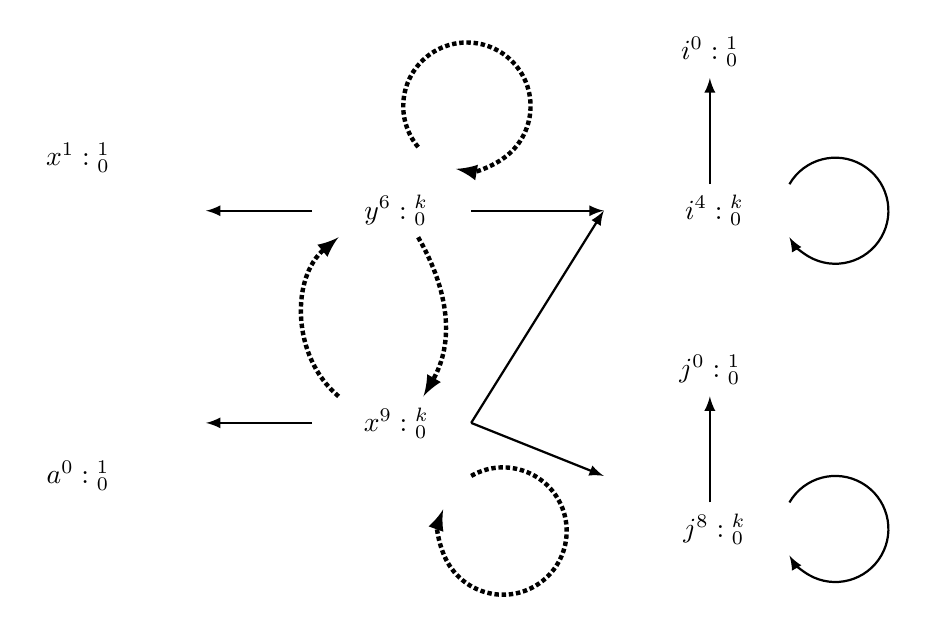
\begin{tikzpicture}[scale=\textwidth/18cm,samples=200]
% Variables Initialization
\draw[] (-6, 1) circle (0pt) node{{ $a^0: {}^1_{0}$}};
\draw[] (-6, 7) circle (0pt) node{{ $x^1: {}^{1}_{0}$}};
% Variables Inside the Loop
   \draw[] (0, 6) circle (0pt) node{{ $y^6: {}^{k}_{0}$}};
   \draw[] (0, 2) circle (0pt) node{{ $x^9: {}^{k}_{0}$}};
   % Counter Variables
   \draw[] (6, 9) circle (0pt) node {{$i^0: {}^{1}_{0}$}};
   \draw[] (6, 6) circle (0pt) node {{ $i^4: {}^{k}_{0}$}};
   \draw[] (6, 3) circle (0pt) node {{$j^0: {}^{1}_{0}$}};
   \draw[] (6, 0) circle (0pt) node {{ $j^8: {}^{k}_{0}$}};
   %
   % Value Dependency Edges:
   \draw[ ultra thick, -latex, densely dotted,] (0.5, 7.2) arc (220:-100:1.2);
   \draw[ thick, -latex] (6, 6.5)  -- (6, 8.5) ;
   \draw[ thick, -latex] (6, 0.5)  -- (6, 2.5) ;
   \draw[ ultra thick, -latex, densely dotted,] (1.5, 1.0) arc (120:-200:1.2);
   % Value Dependency Edges on Initial Values:
   \draw[ thick, -latex,] (-1.5, 2)  -- (-3.5, 2) ;
   \draw[ thick, -latex,] (-1.5, 6)  -- (-3.5, 6) ;
   %
   \draw[ ultra thick, -latex, densely dotted,] (-1, 2.5)  to  [out=-220,in=220]  (-1, 5.5);
   \draw[ ultra thick, -latex, densely dotted,]  (0.5, 5.5) to  [out=-60,in=60] (0.6, 2.5) ;
   % Control Dependency
  %  \draw[ thick,-latex] (1.5, 7)  -- (4, 9) ;
  %  \draw[ thick,-latex] (1.5, 4)  -- (4, 9) ;
  \draw[ thick, -latex, ] (7.5, 6.5) arc (150:-150:1);
  \draw[ thick, -latex, ] (7.5, 0.5) arc (150:-150:1);
  \draw[ thick,-latex] (1.5, 6)  -- (4, 6) ;
   \draw[ thick,-latex] (1.5, 2)  -- (4, 6) ;
   \draw[ thick,-latex] (1.5, 2)  -- (4, 1) ;
   \end{tikzpicture}
   \caption{}
      \end{centering}
      \end{subfigure}
    }
    \vspace{-0.4cm}
     \caption{(a) The nested while loop example, (b) The estimated dependency graph generated from $\THESYSTEM$.}
    \label{fig:alg_adaptsearch_nestedwhile}
    \end{figure}
    %
        \begin{algorithm}
          \caption{
          {Over-Approximated Adaptivity on SCC}
          \label{alg:overadp_alg}
          }
          \begin{algorithmic}[1]
          \REQUIRE $G = (\vertxs, \edges, \weights, \qflag)$ \#\{An Strong Connected Symbolic Weighted Directed Graph\}
          \STATE {\bf {$\kw{\pathsearch_{scc-naive}(G)}$}:}  
          \STATE {\bf init} 
          \\
          $\kw{r_{scc}}$: the Adaptivity of this SCC
          \STATE  {\bf for} every vertex $v$ in $\vertxs$:
          \STATE  \qquad $\kw{r_{scc}} += \weights(v)*\qflag(v)$  
          \RETURN $r[c]$
          \end{algorithmic}
          \end{algorithm}
          %